

\section{Additional diversity analysis}%

\label{app:additional_diversity_analysis}
\subsection{On OfficeHome}

\subsubsection{Feature diversity}
\label{app:analysis_office_features}
In \Cref{sect:analysis}, our diversity-based theoretical findings were empirically validated using the ratio-error \cite{aksela2003comparison}, a common diversity measure notably used in \cite{rame2021dice,rame2021ixmo}.
In \Cref{fig:home0_df}, we recover similar conclusions with another diversity measure: the Centered Kernel Alignment Complement (CKAC) \cite{DBLP:journals/corr/abs-1905-00414}, also used in \cite{Neyshabur2020,Wortsman2022robust}.
CKAC operates in the feature space and measures to what extent the pairwise similarity matrices (computed on domain $T$) are aligned --- where similarity is the dot product between penultimate representations extracted from two different networks.
\begin{figure}[h]%
    \centering%
    \begin{subfigure}{.33\textwidth}%
        \centering%
        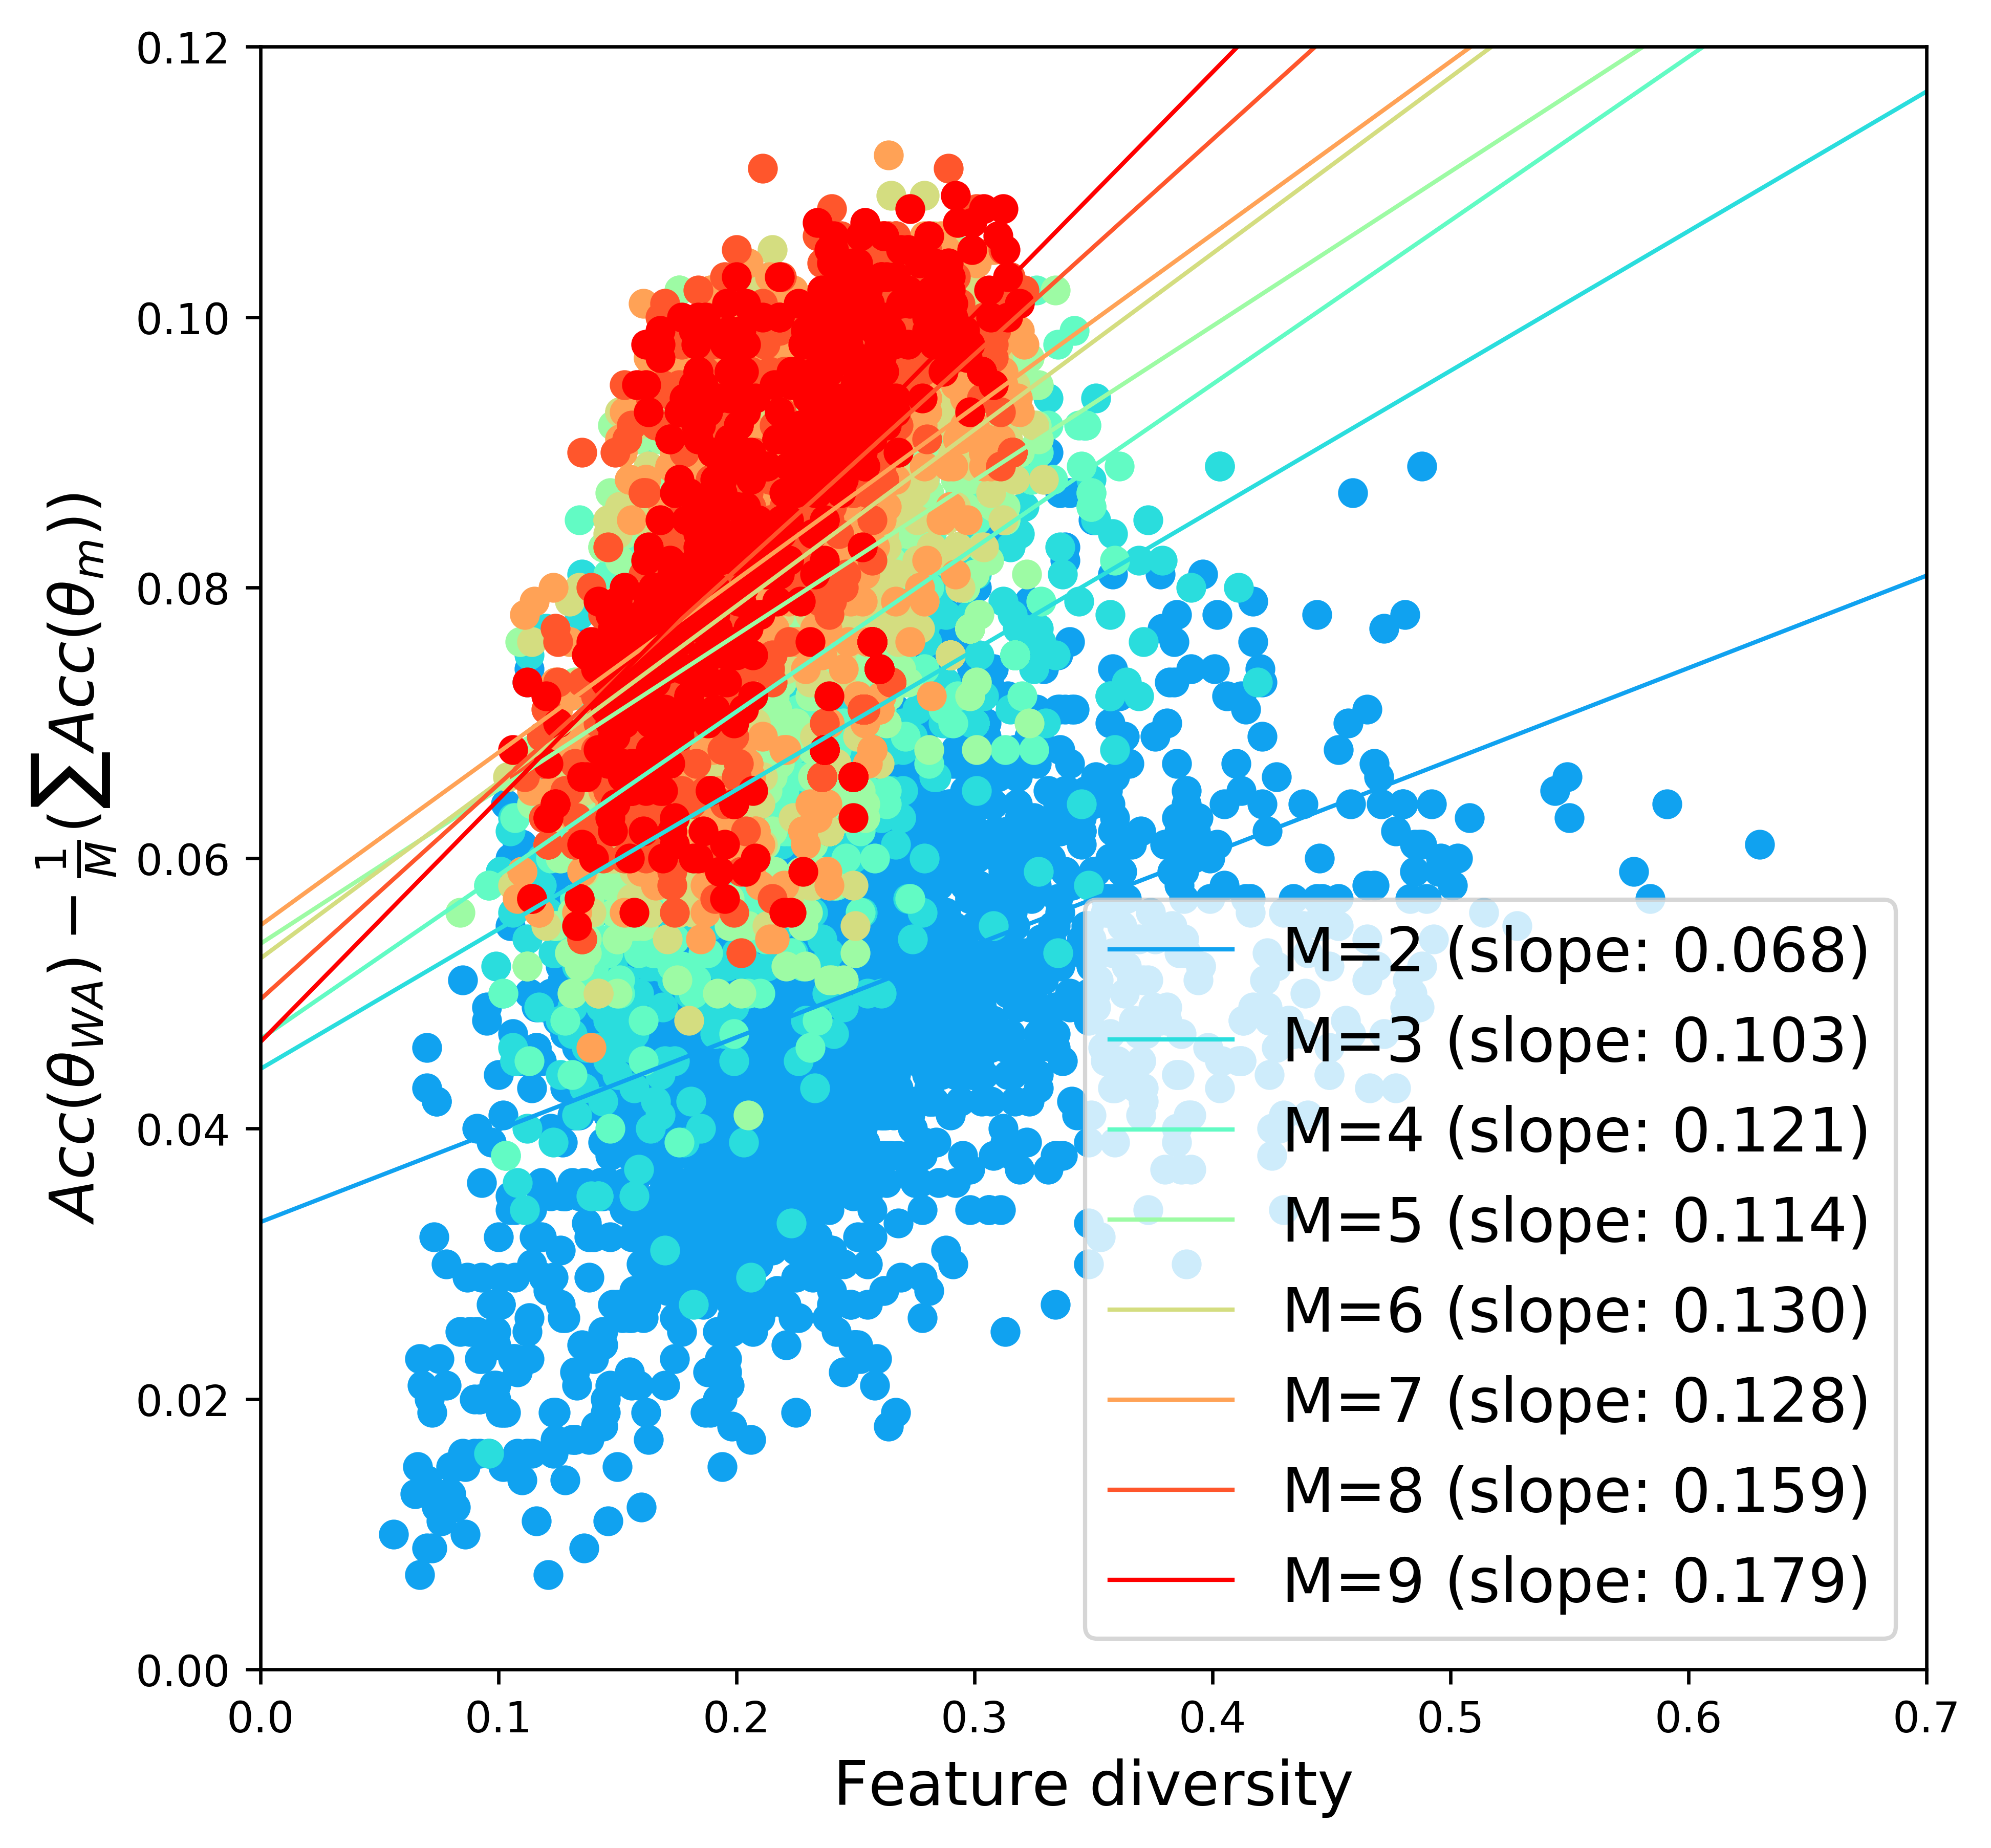
\includegraphics[width=\linewidth]{pictures/files/final/home0_samediffruns_df_soup-netm_77.png}%
        \caption{Same as \Cref{fig:home0_dr_soup-netm}.}%
        \label{fig:home0_df_soup-netm}%
    \end{subfigure}%
    \begin{subfigure}{.33\textwidth}%
        \centering%
        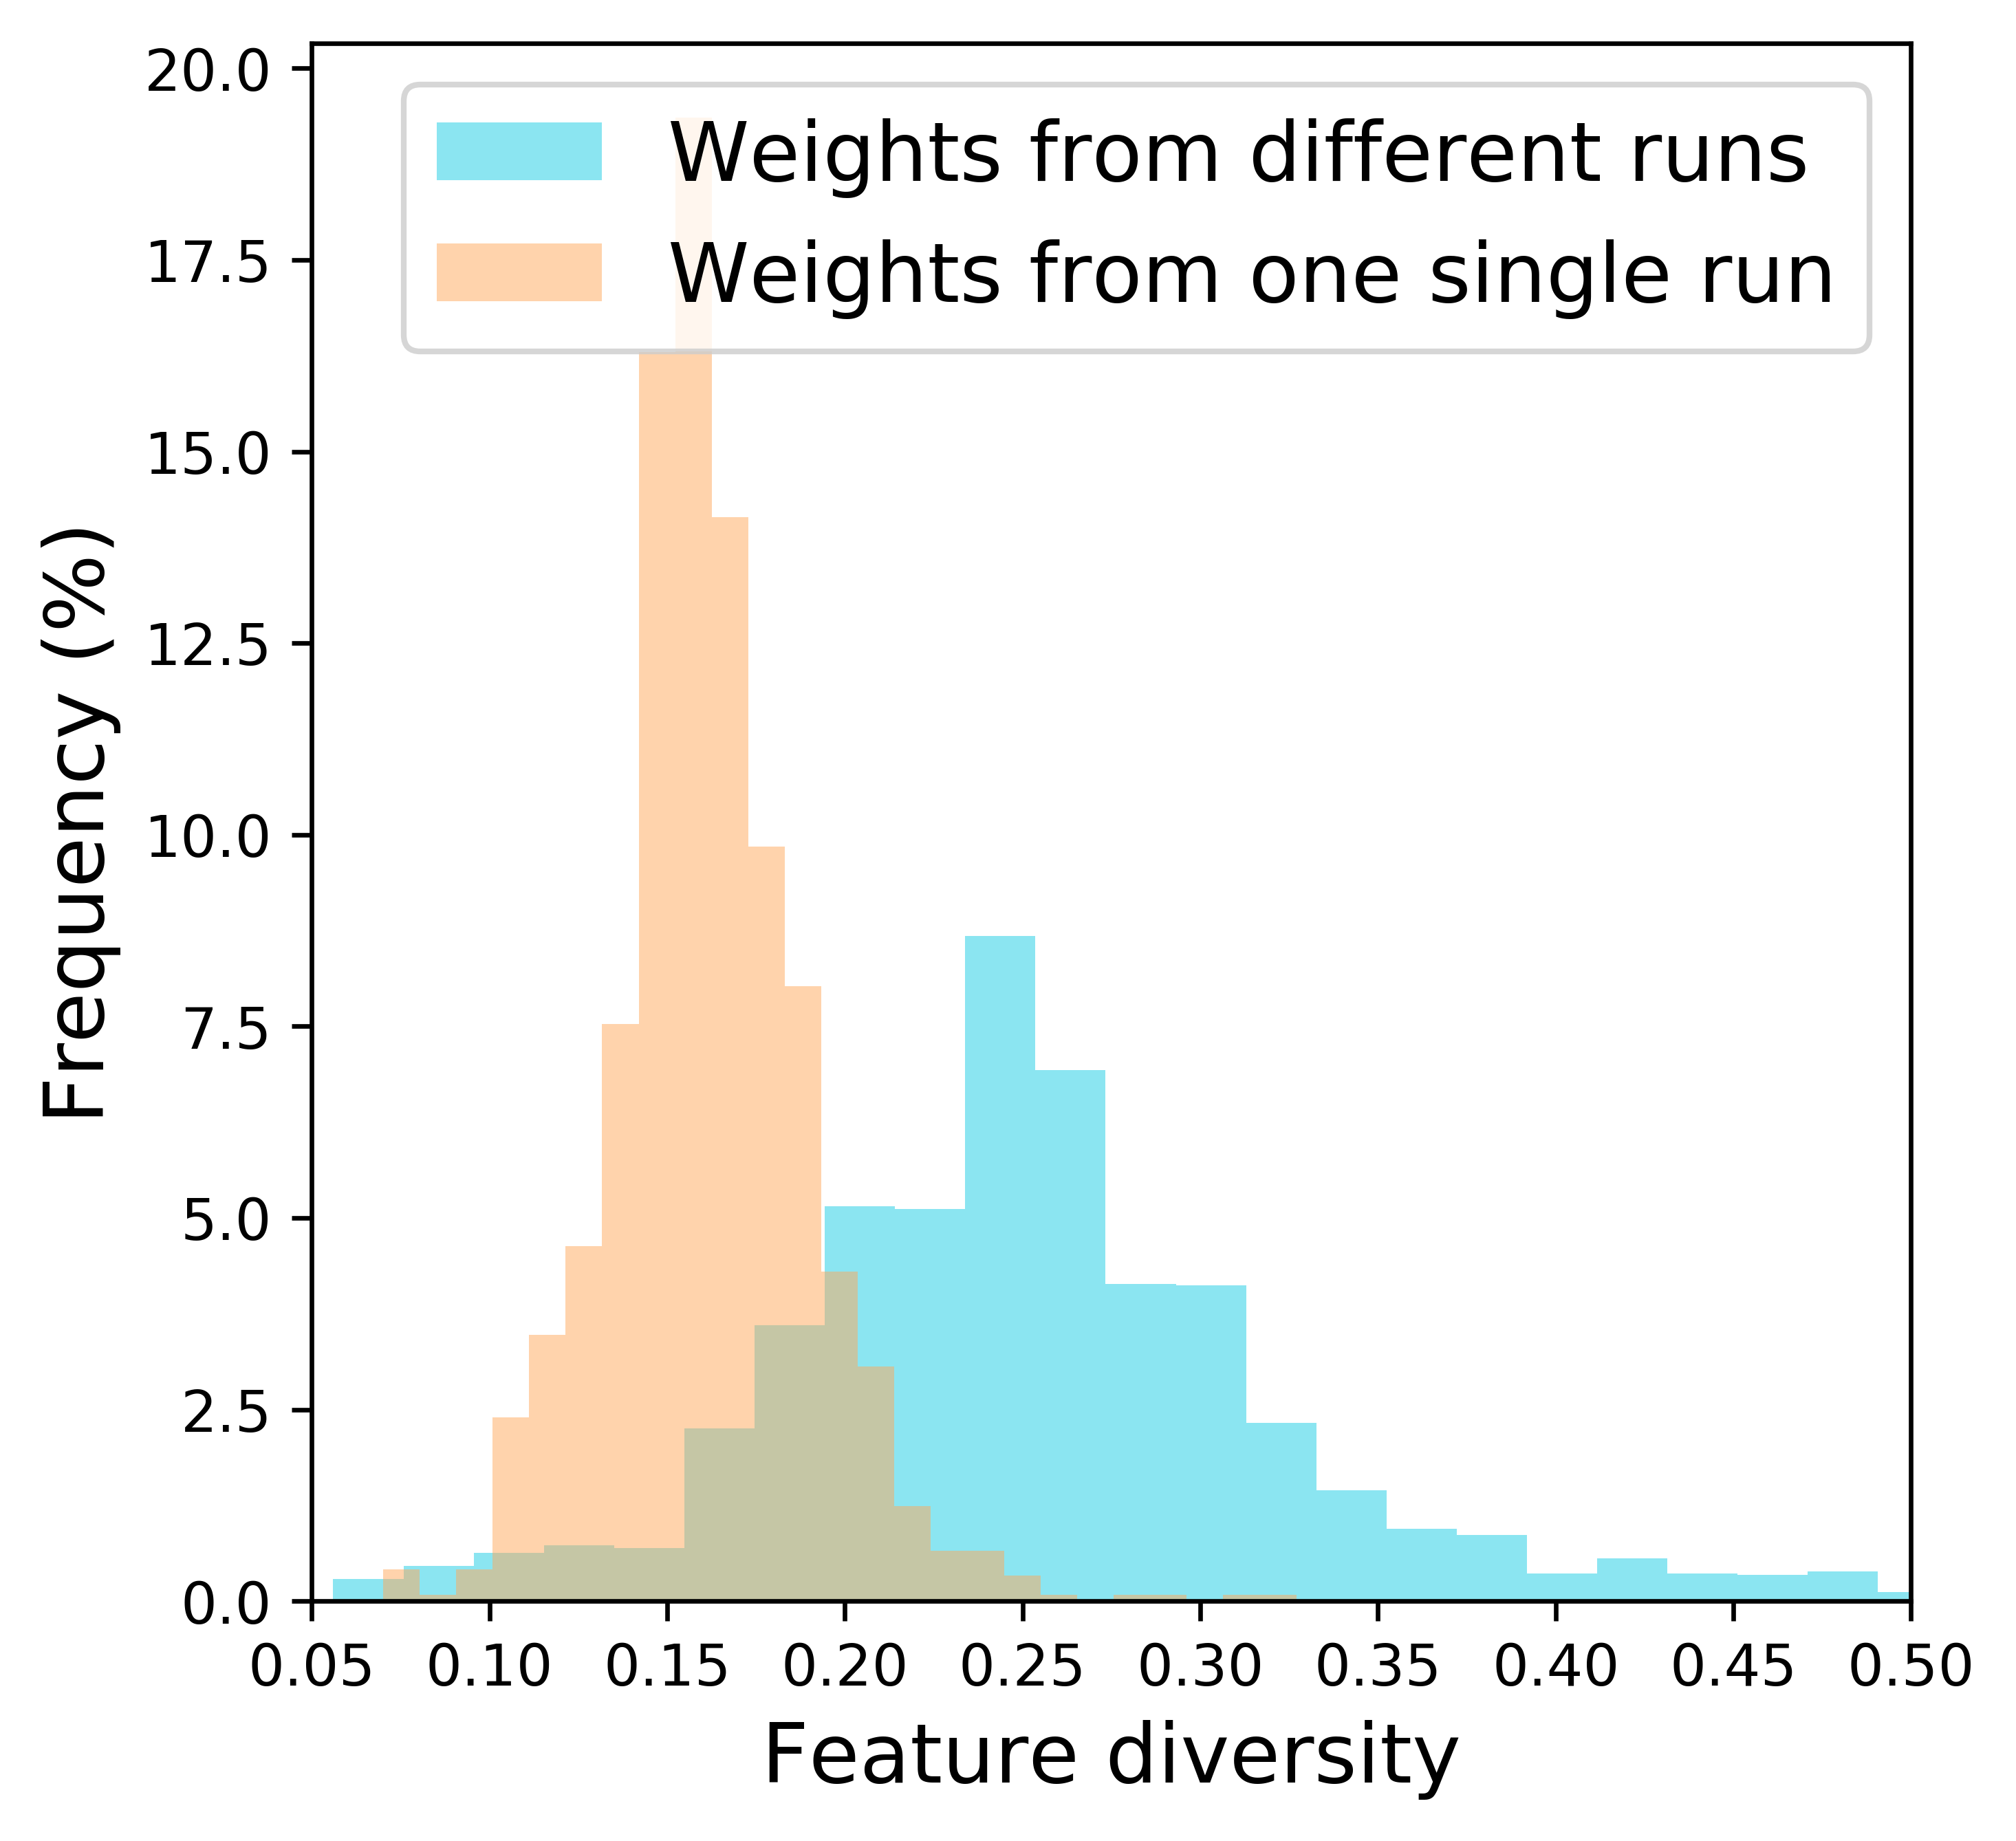
\includegraphics[width=\textwidth]{pictures/files/final/home0_hist_df.png}%
        \caption{Same as \Cref{fig:home0_dr_frequency}.}%
        \label{fig:home0_df_frequency}%
    \end{subfigure}%
    \begin{subfigure}{.33\textwidth}%
        \centering%
        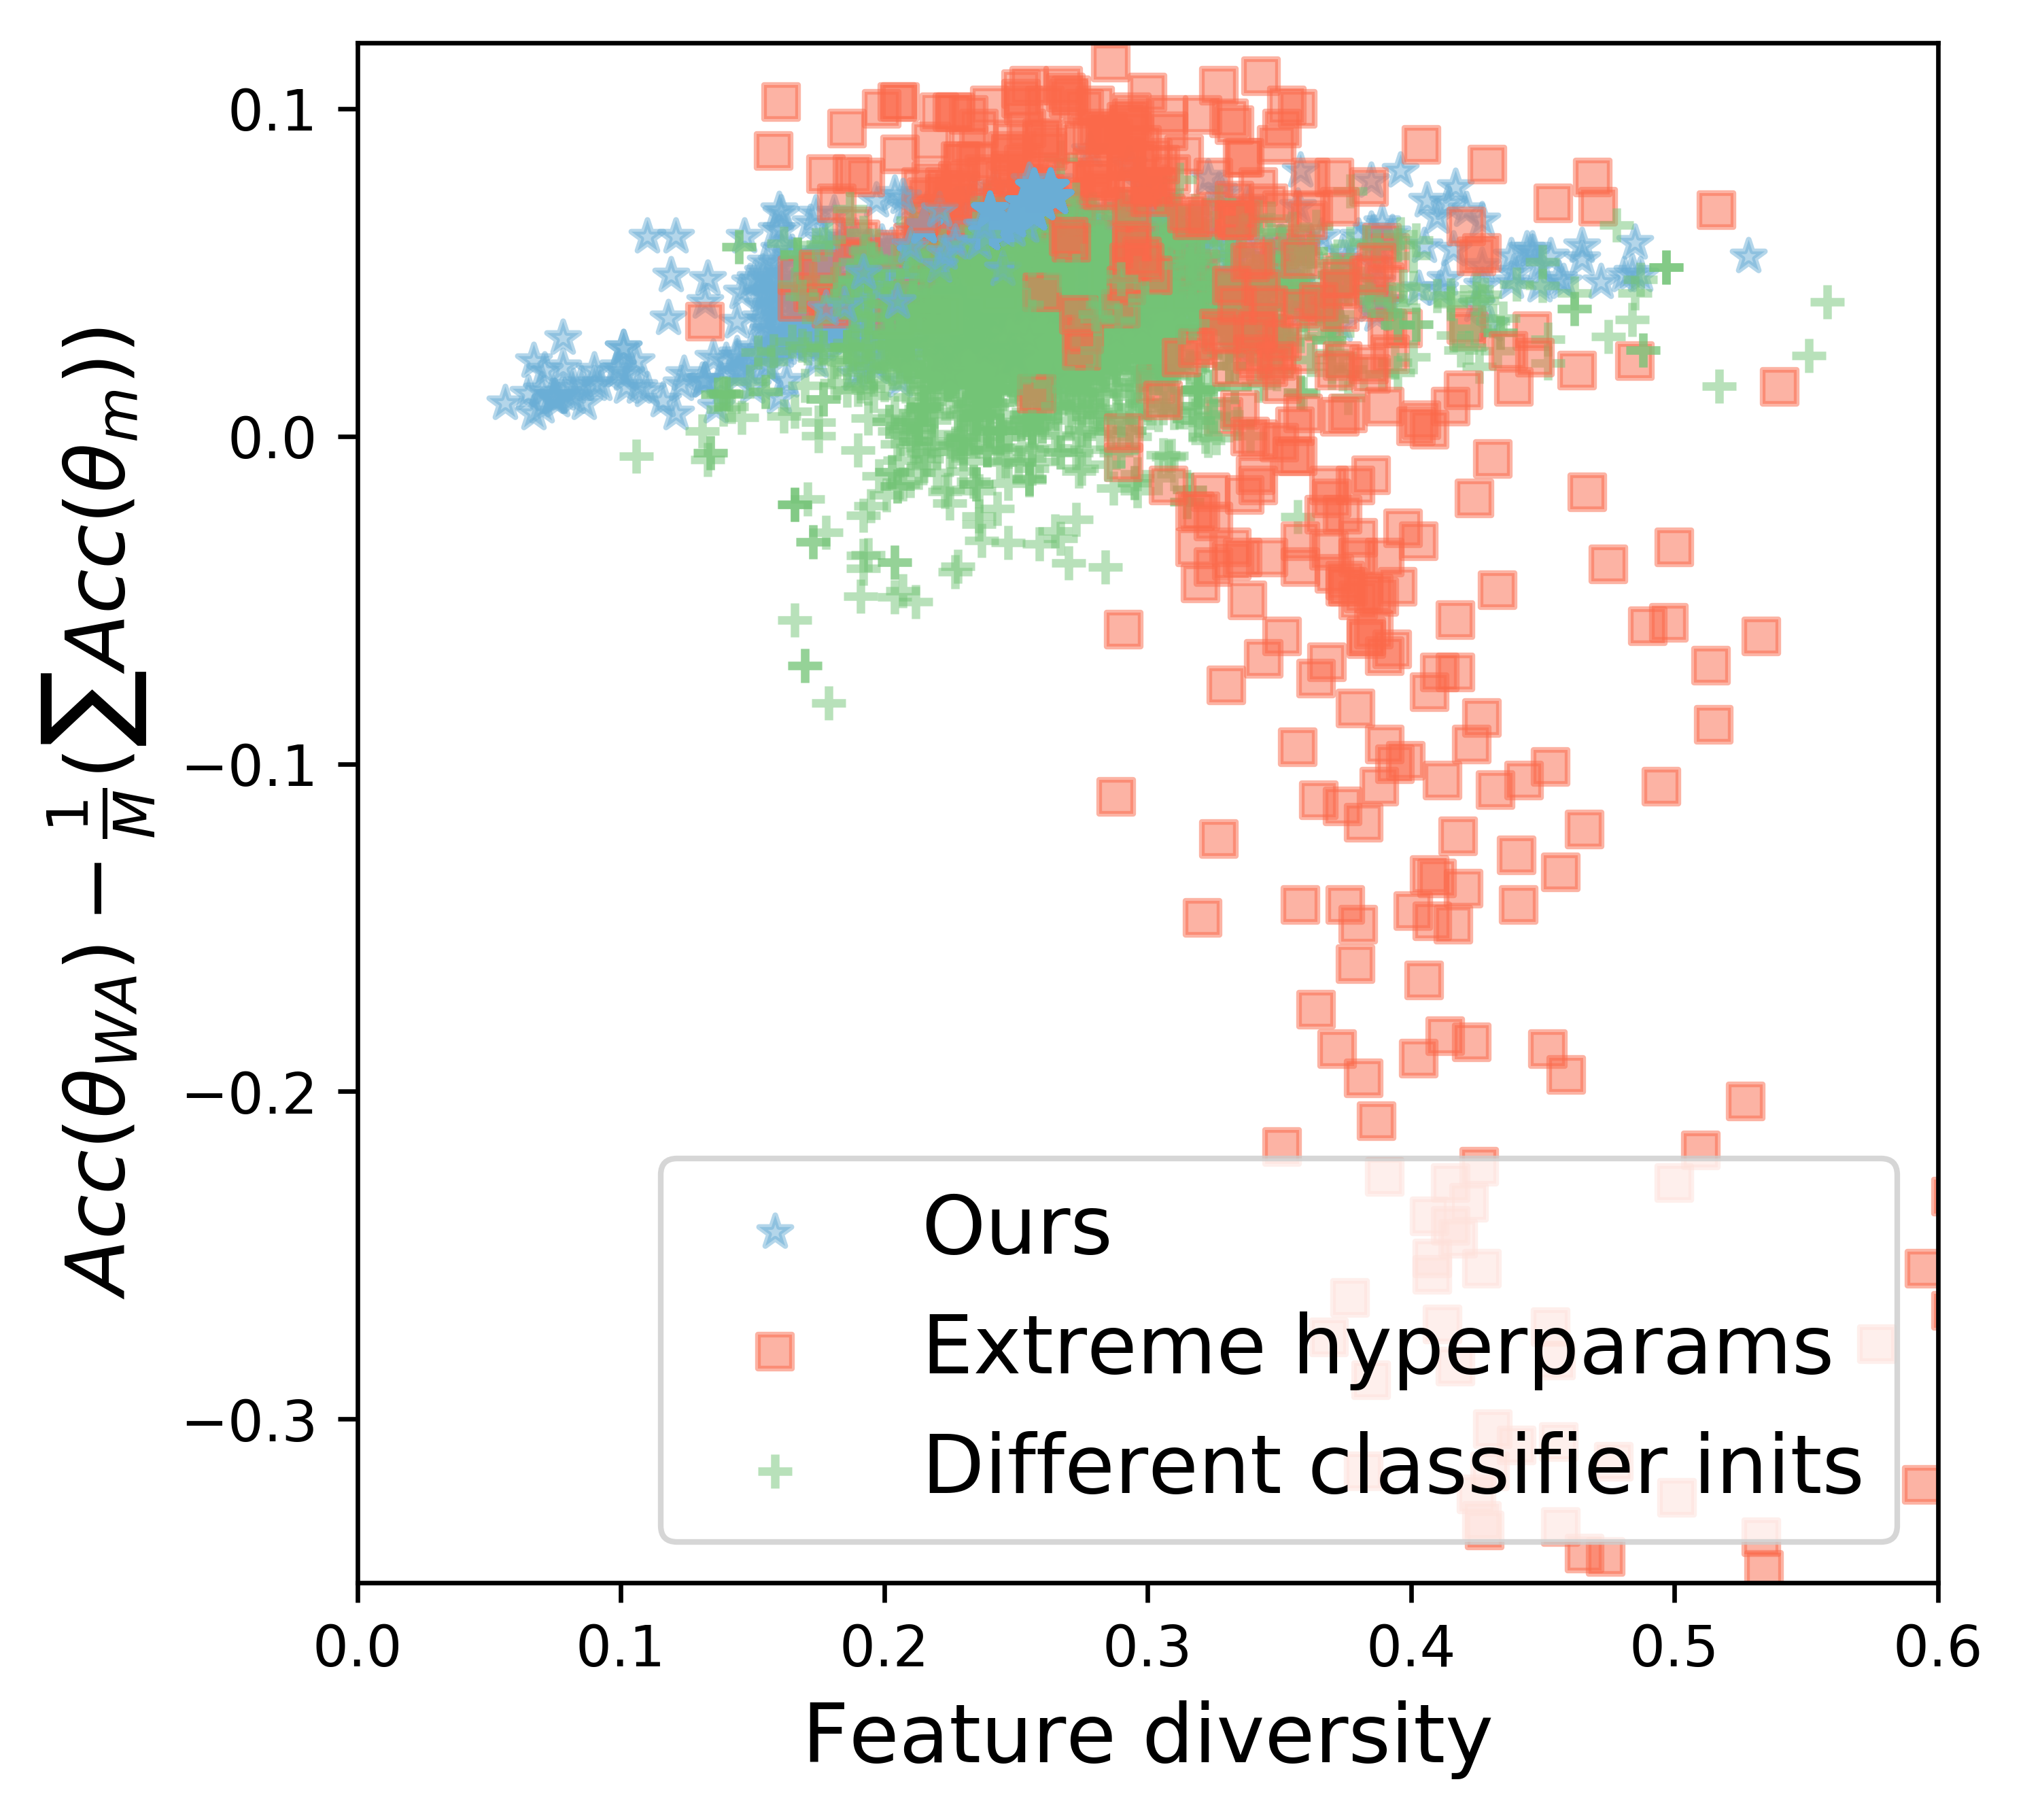
\includegraphics[width=\linewidth]{pictures/files/final/home0_diffrunslargehpnosh_df_soup-netm.png}%
        \caption{Same as \Cref{fig:home0_locality_requirement}.}%
        \label{fig:home0_locality_requirement_df}%
    \end{subfigure}%
    \caption{Same analysis as \Cref{sect:analysis}, where diversity is measured with CKAC \cite{DBLP:journals/corr/abs-1905-00414} in features rather than with ratio-error \cite{aksela2003comparison} in predictions.}%
    \label{fig:home0_df}%
\end{figure}%%
\subsubsection{Accuracy gain per unit of diversity}
\label{app:soup:m_slope}
In \Cref{fig:home0_dr_soup-netm,fig:home0_df_soup-netm}, we indicated the slope of the linear regressions relating diversity to accuracy gain at fixed $M$ (between $2$ and $9$).
For example, when $M=9$ weights are averaged, the accuracy gain increases by $0.297$ per unit of additional diversity in prediction  \cite{aksela2003comparison} (see \Cref{fig:home0_dr_soup-netm}) and by $0.179$ per unit of additional diversity in features \cite{DBLP:journals/corr/abs-1905-00414} (see \Cref{fig:home0_df_soup-netm}).
Most importantly, we note that the slope increases with $M$.
To make this more visible, we plot slopes \wrt $M$ in \Cref{fig:soup:m_slope}.
Our observations are consistent with the $(M-1)/M$ factor in front of $\covb\left(x\right)$ in \Cref{eq:b_var_cov}.
This shows that diversity becomes more important for large $M$.
Yet, large $M$ is computationally impractical in standard functional ensembling, as one forward step is required per model.
In contrast, WA has a fixed inference time which allows it to consider larger $M$. Increasing $M$ from $20$ to $60$ is the main reason why DiWA$^{\dagger}$ improves DiWA.
\begin{figure}[H]
    \centering%
    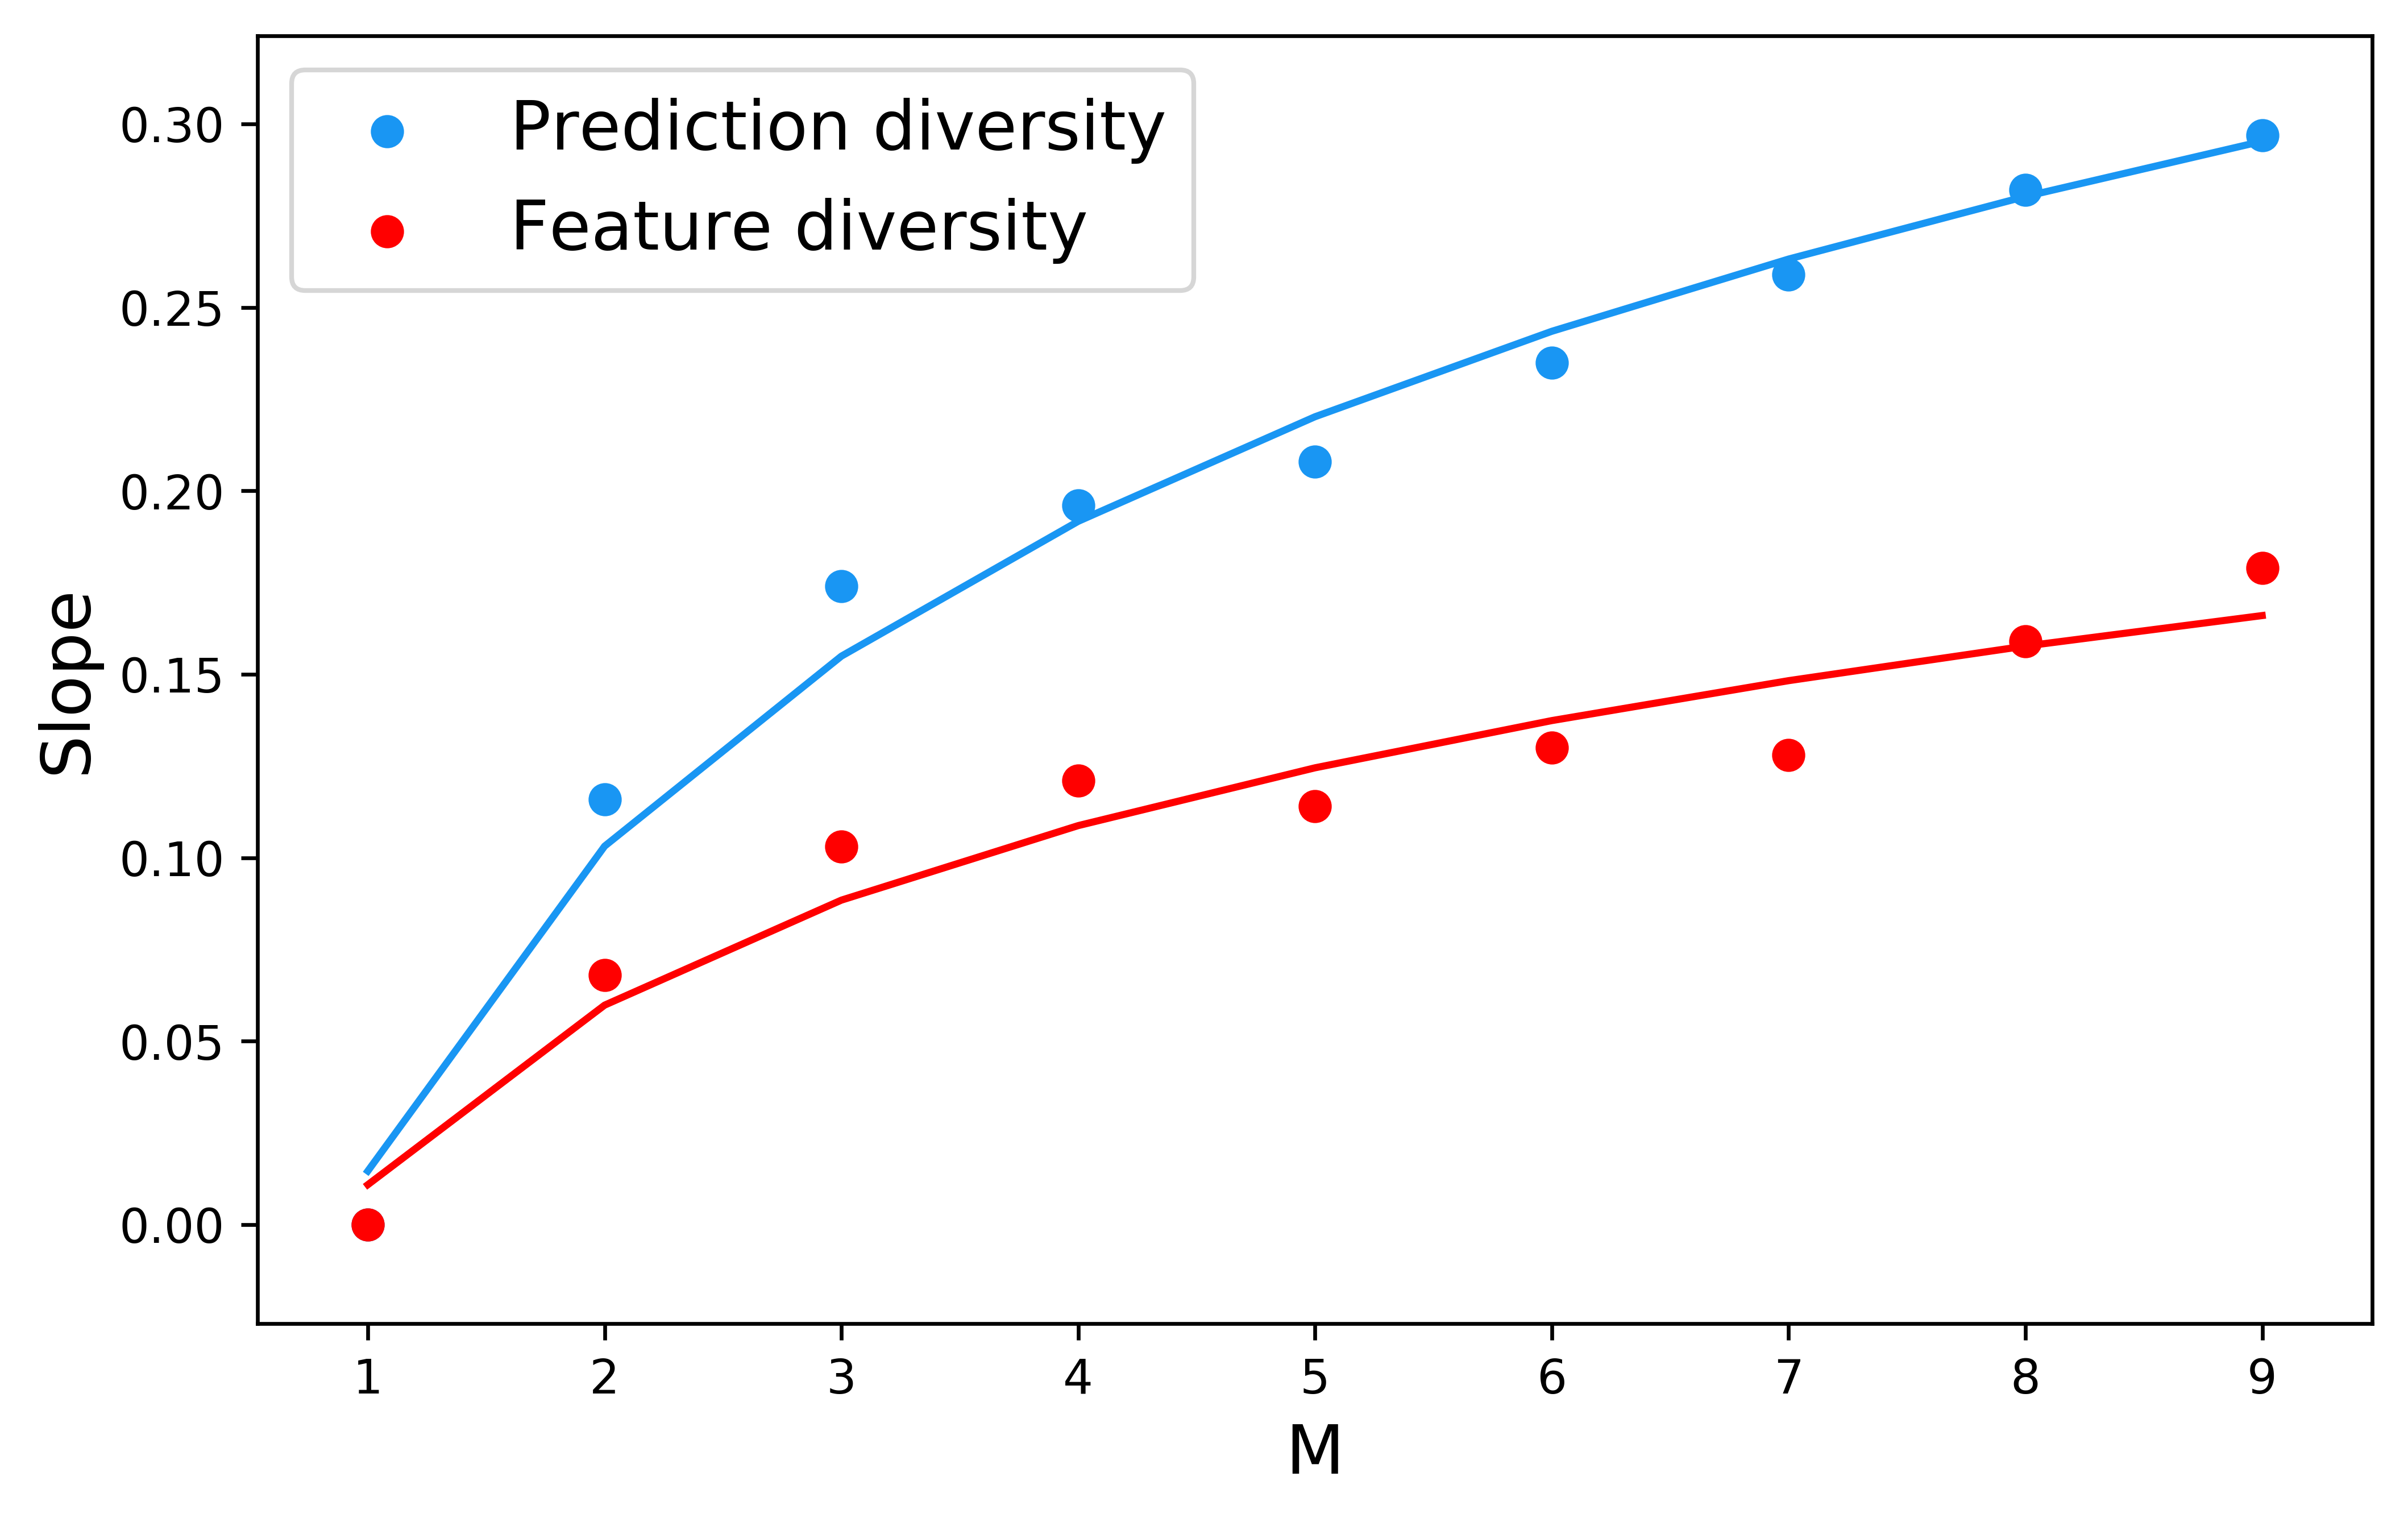
\includegraphics[width=0.5\textwidth]{pictures/files/final/home0_m_slope.png}%
    \caption{The slopes of linear regression --- relating diversity to accuracy gain in \Cref{fig:home0_dr_soup-netm} and \Cref{fig:home0_df_soup-netm} --- increases with $M$.}
    \label{fig:soup:m_slope}%
\end{figure}%

% \begin{wrapfigure}[15]{hR!}{0.34\textwidth}
%     % \vspace{-3em}%
%     \centering%
%     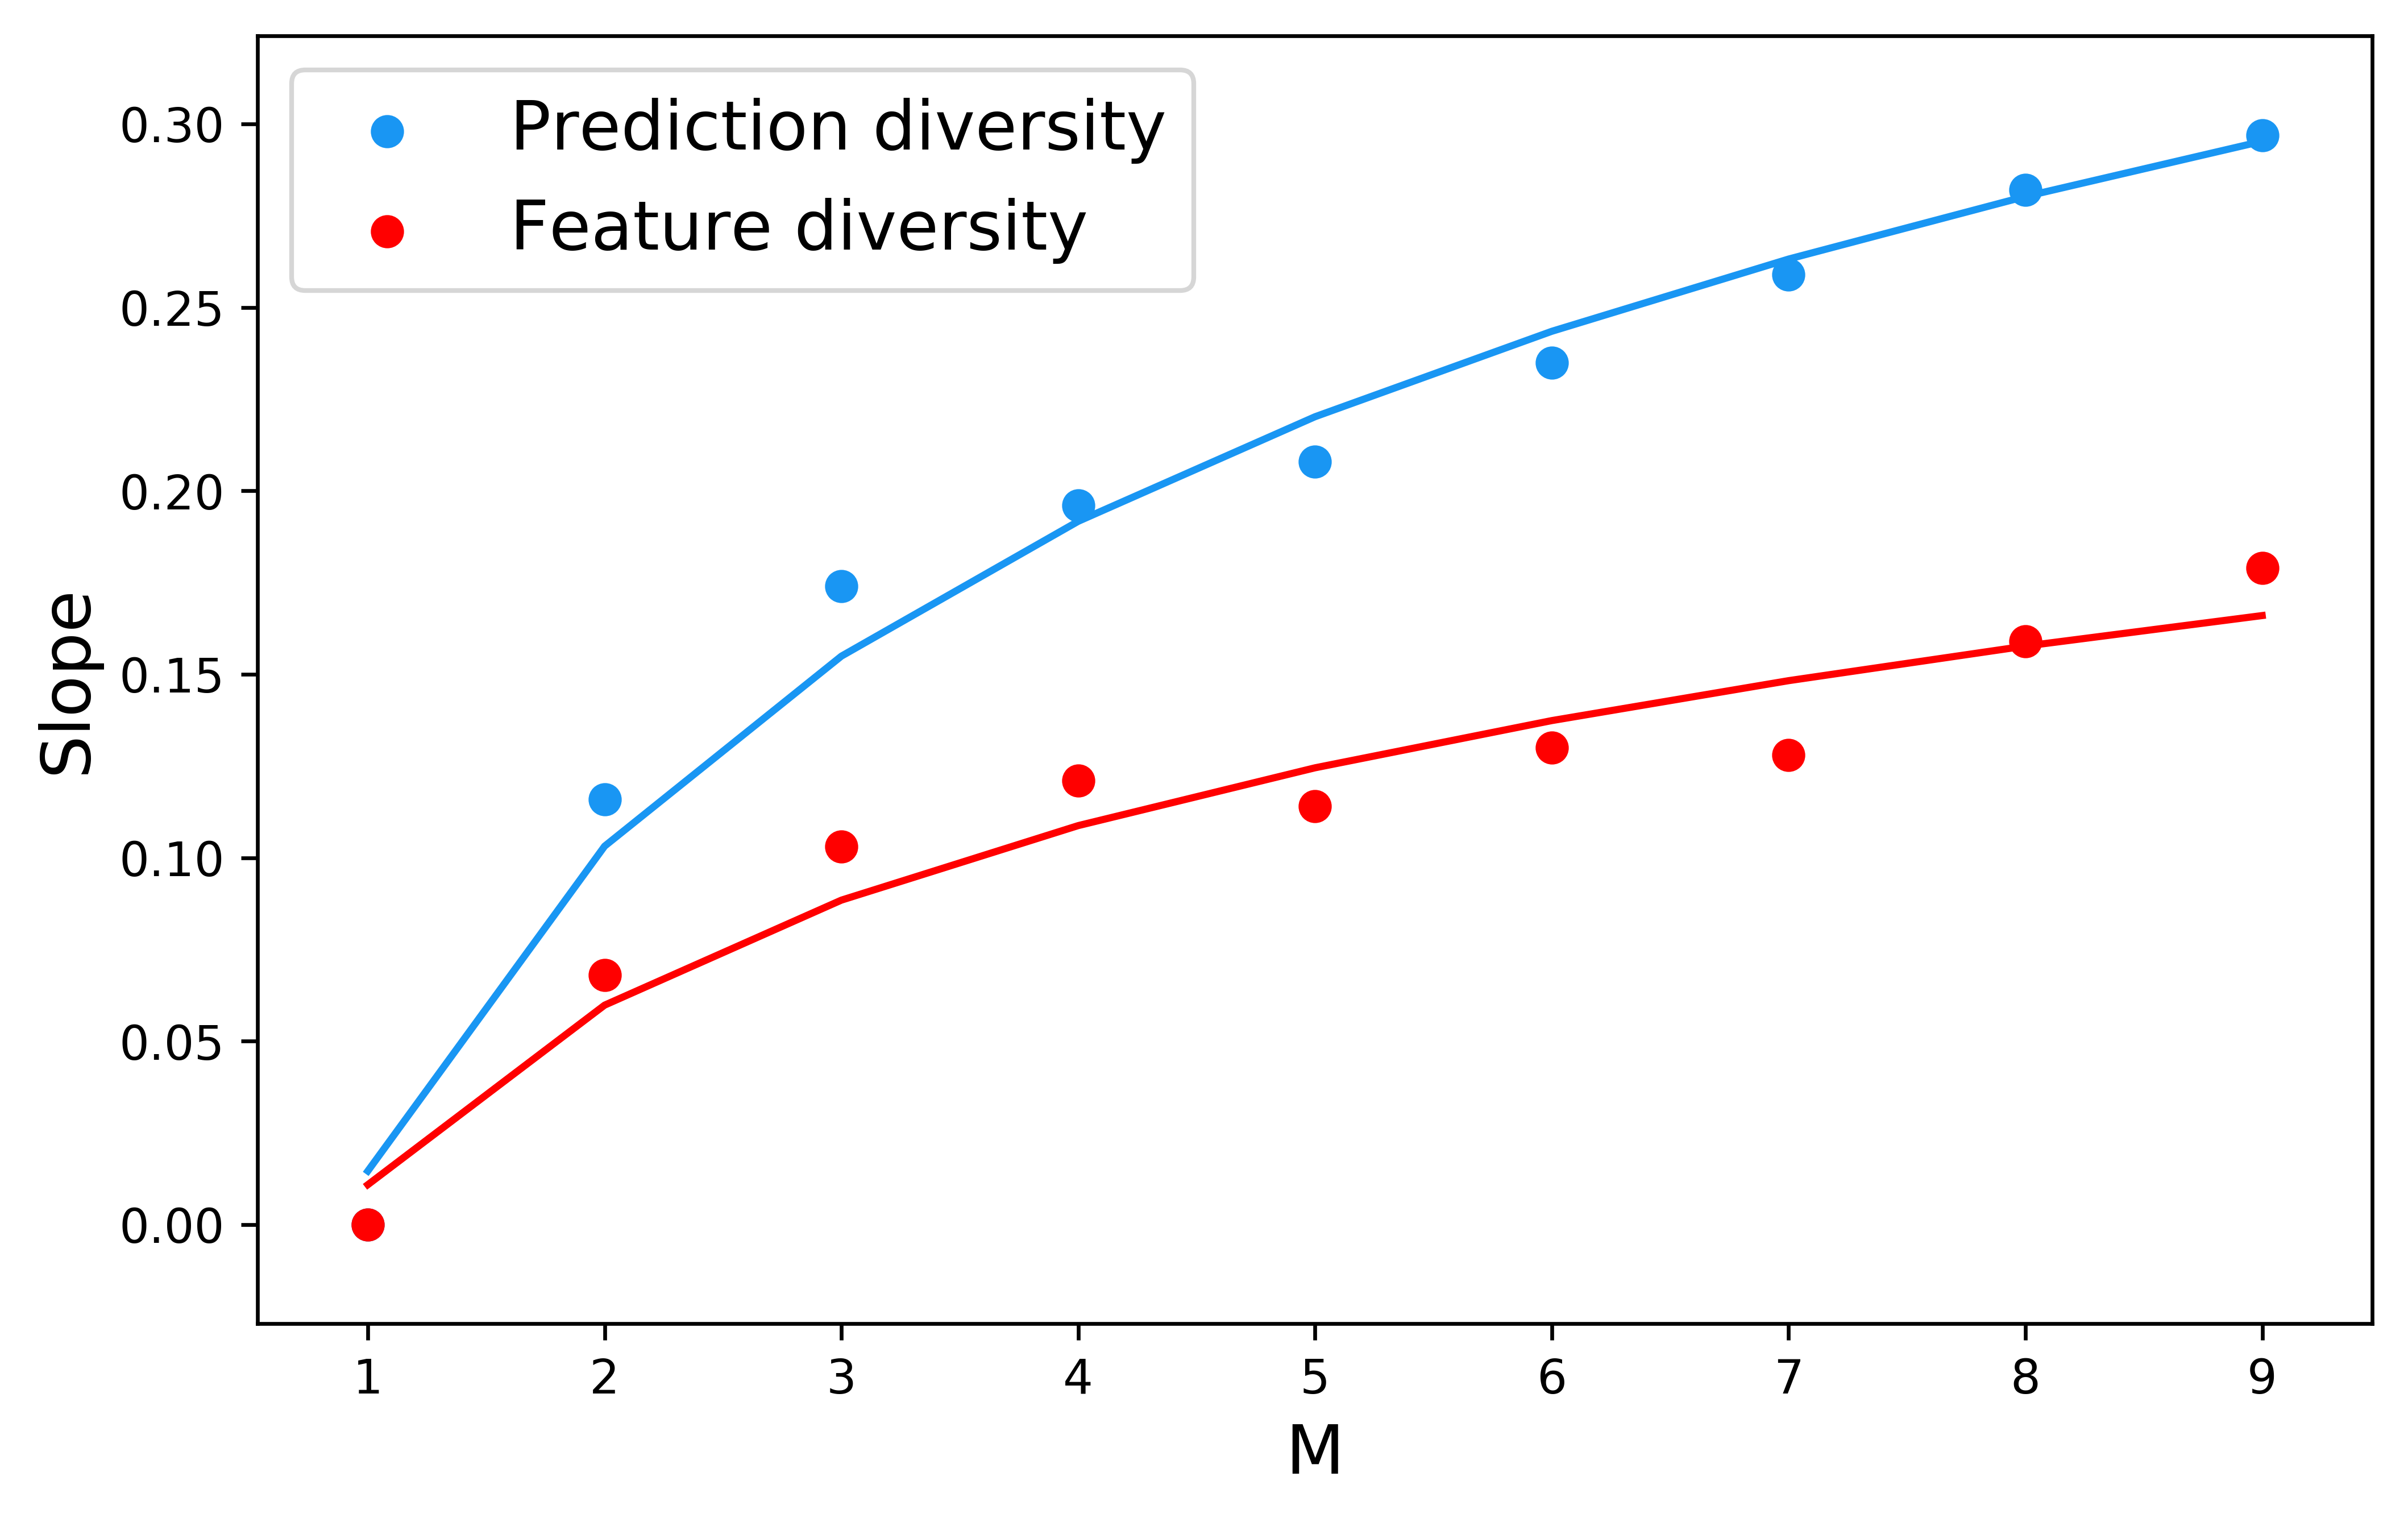
\includegraphics[width=0.5\textwidth]{pictures/files/final/home0_m_slope.png}%
%     \caption{The slopes of linear regressions --- relating diversity to accuracy gain in \Cref{fig:home0_dr_soup-netm} and \Cref{fig:home0_df_soup-netm} --- increases with $M$.}
%     \label{fig:soup:m_slope}%
%     % \vspace{-3em}
% \end{wrapfigure}%
\subsubsection{Diversity comparison across a wide range of methods}
\label{app:more_diversity_comparison}
Inspired by \cite{gontijolopes2022no}, we further analyze in \Cref{fig:home0_boxplot} the diversity between two weights obtained from different (more or less correlated) learning procedures.
\begin{itemize}
    \item In the upper part, weights are obtained from a single run. They share the same initialization/hyperparameters/data/noise in the optimization procedure and only differ by the number of training steps (which we choose to be a multiple of $50$). They are less diverse than the weights in the middle part of \Cref{fig:home0_boxplot}, that are sampled from two ERM runs.
    \item  When sampled from different runs, the weights become even more diverse when they have more extreme hyperparameter ranges, they do not share the same classifier initialization or they are trained on different data. The first two are impractical for WA, as it breaks the locality requirement (see \Cref{fig:home0_locality_requirement,fig:home0_locality_requirement_df}).
          Luckily, the third setting \enquote{data diversity} is more convenient and is another reason for the success of DiWA$^{\dagger}$; its $60$ weights were trained on $3$ different data splits. Data diversity has provable benefits \cite{efron1992bootstrap}, \eg in bagging \cite{breiman1996bagging}.
    \item Finally, we observe that diversity is increased (notably in features) when two runs have different objectives, for example, Interdomain Mixup \cite{yan2020improve} and Coral \cite{coral216aaai}. Thus incorporating weights trained with different invariance-based objectives have two benefits that explain the strong results in \Cref{table:db_home0_training}: (1) they learn invariant features by leveraging the domain information and (2) they enrich the diversity of solutions by extracting different features. These solutions can bring their own particularity to WA.
\end{itemize}
In conclusion, our analysis confirms that \enquote{model pairs that diverge more in training methodology display categorically different generalization behavior, producing increasingly uncorrelated errors}, as stated in \cite{gontijolopes2022no}.
\begin{figure}[h]%
    \centering%
    \begin{subfigure}{.5\textwidth}%
        \centering%
        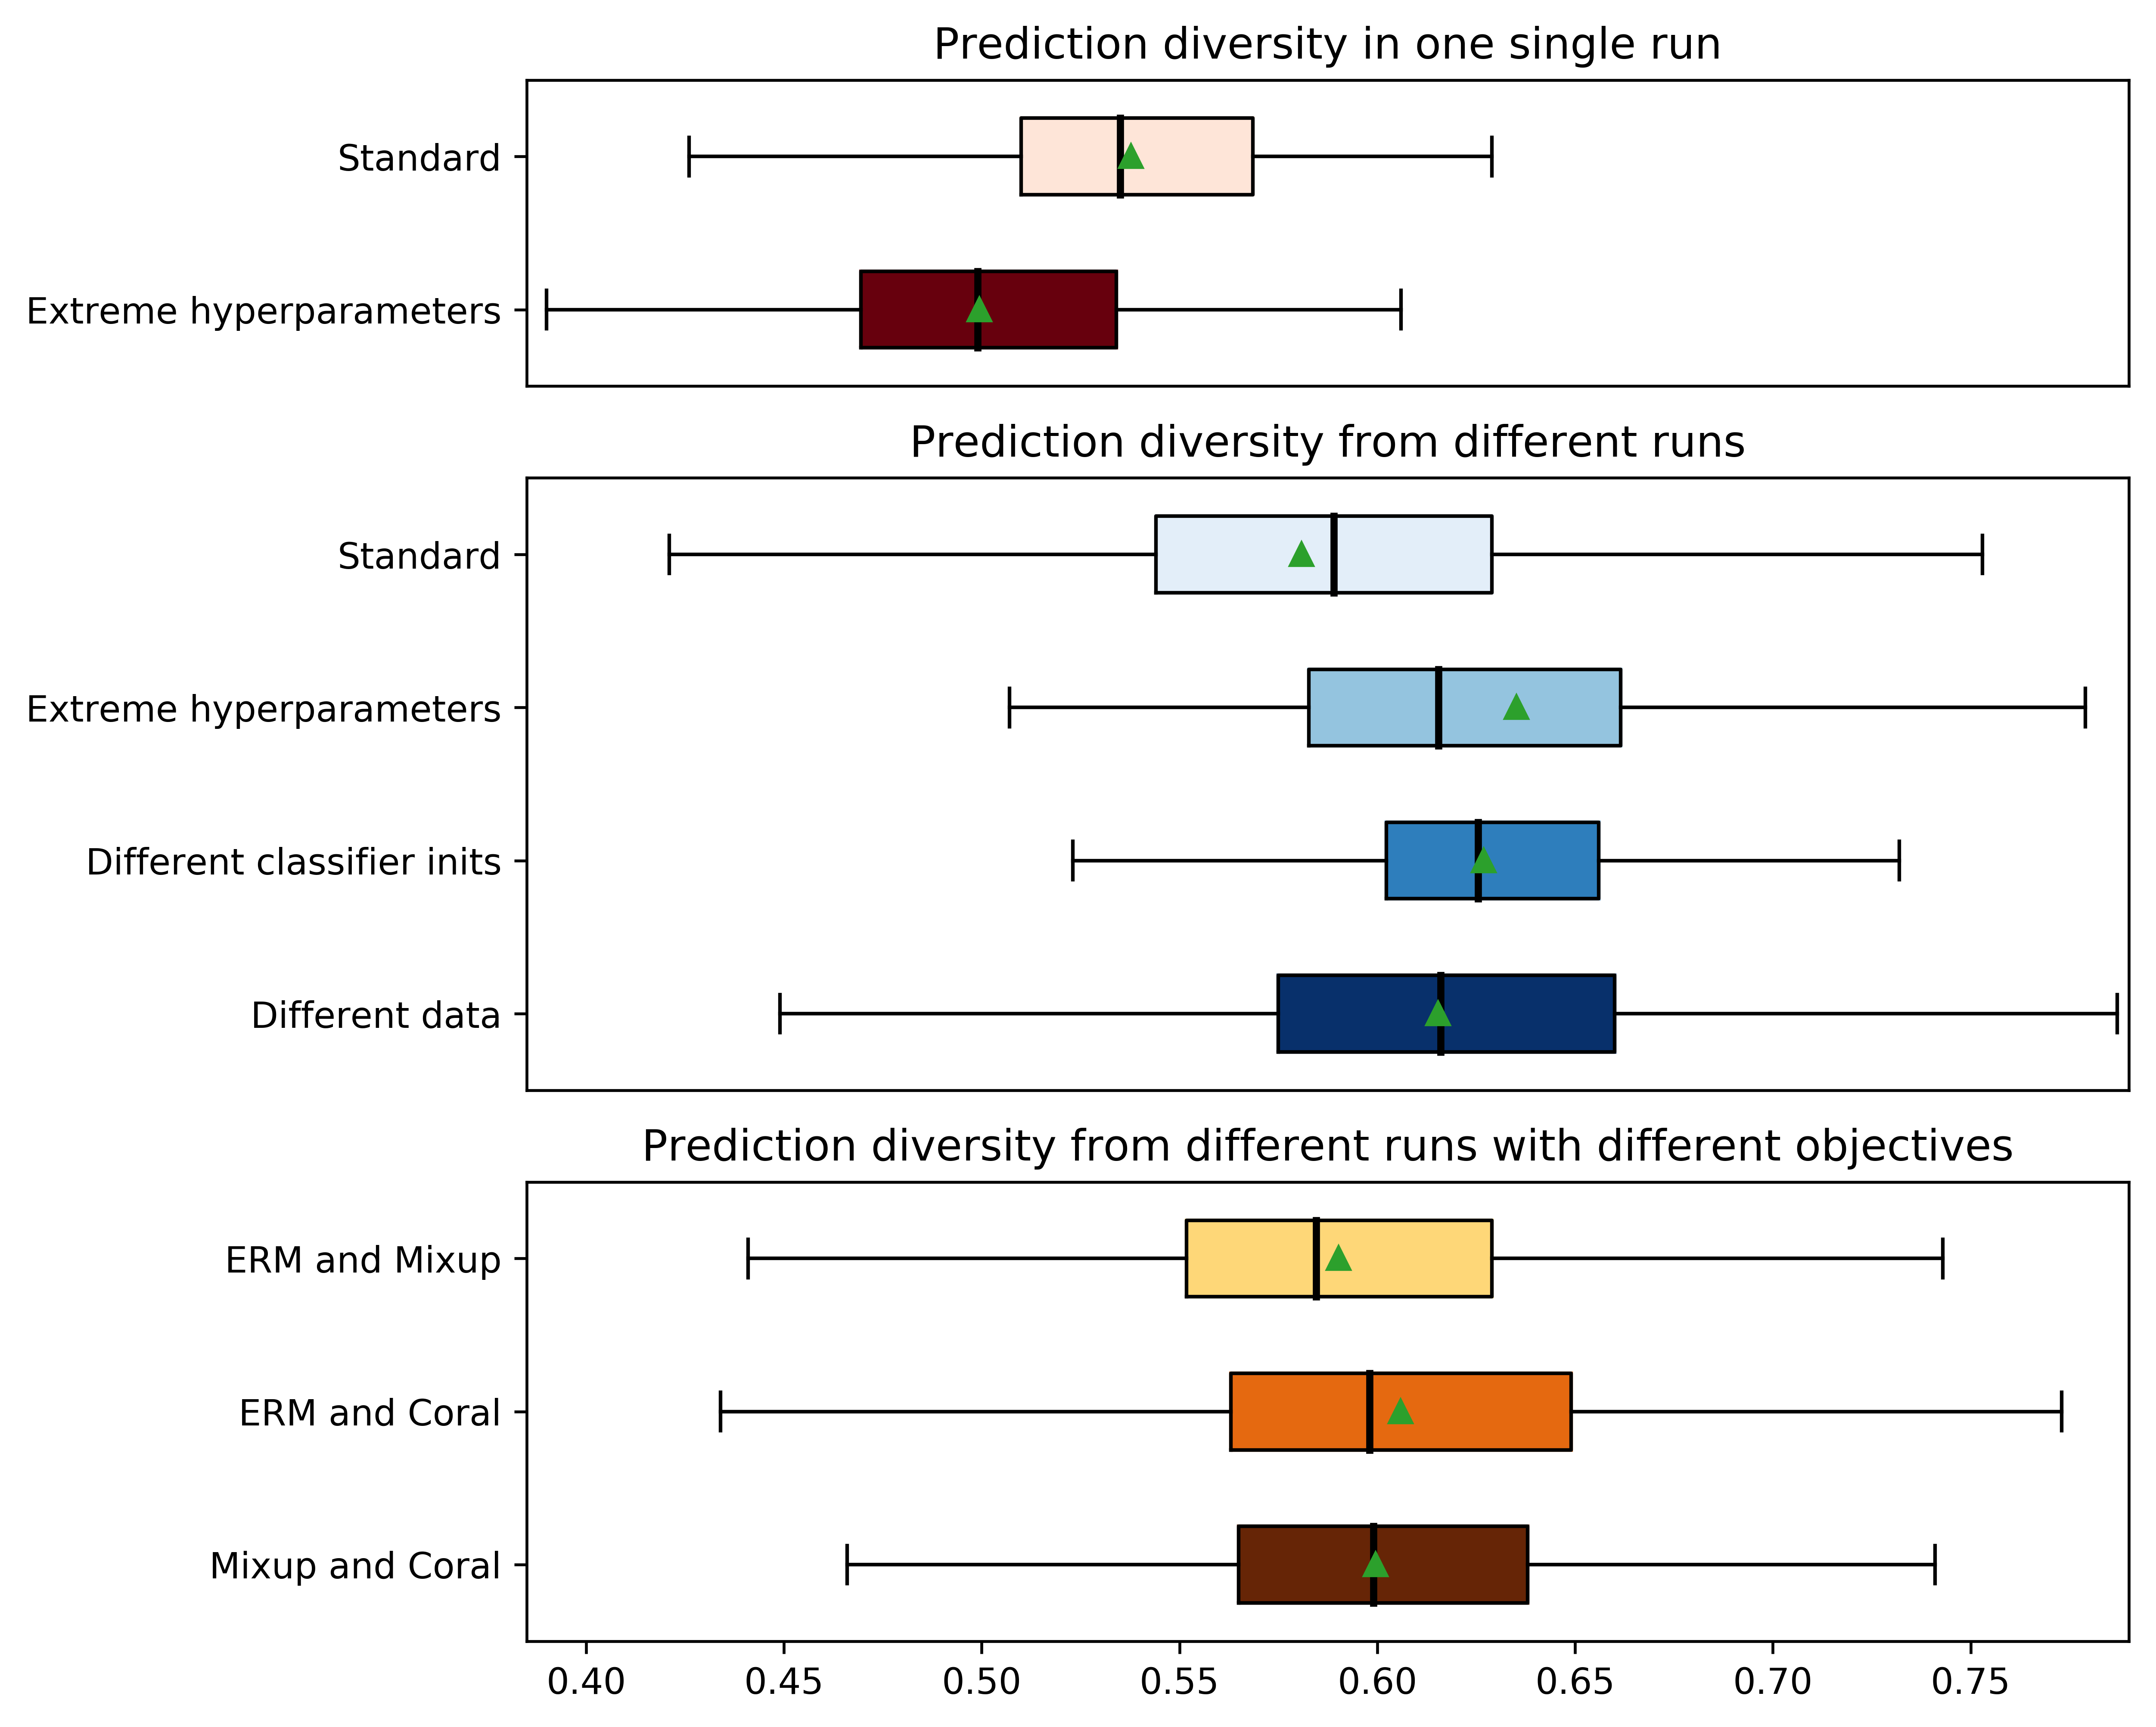
\includegraphics[width=1.0\textwidth]{pictures/files/final/boxplot_dr.png}%
        \caption{Prediction diversity \cite{aksela2003comparison}.}
        \label{fig:home0_dr_boxplot}%
    \end{subfigure}%
    \begin{subfigure}{.5\textwidth}%
        \centering%
        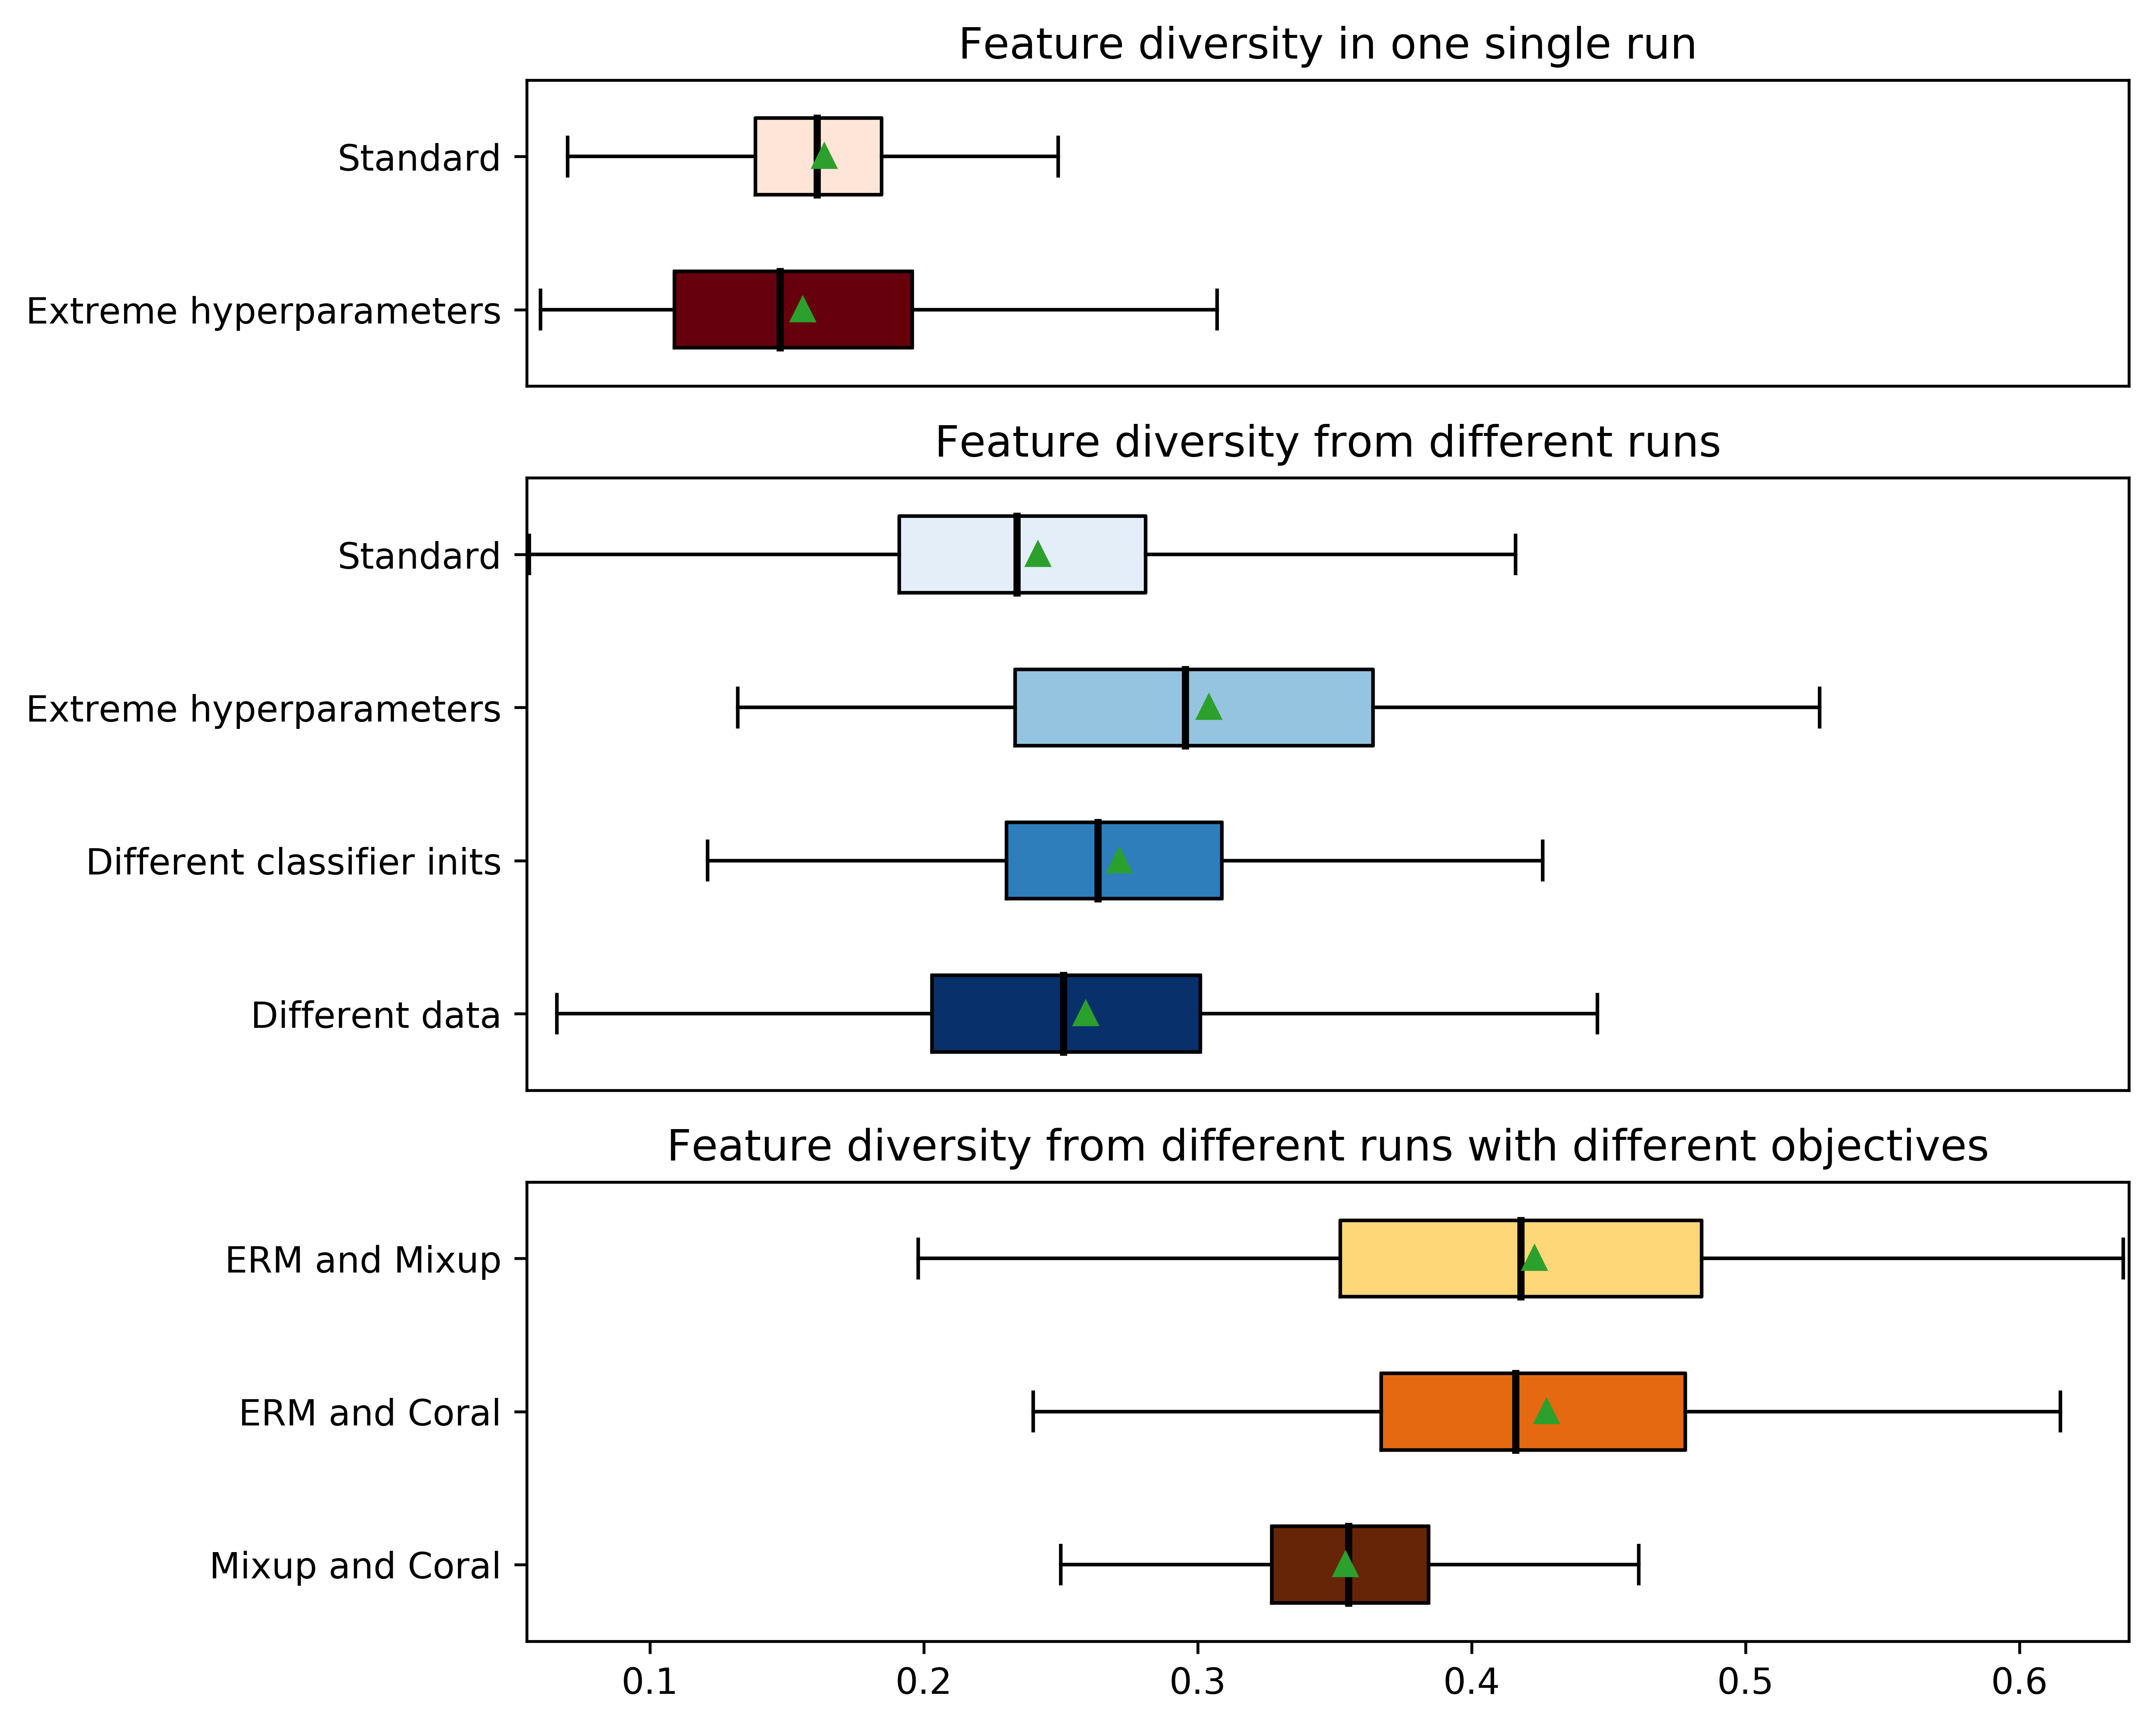
\includegraphics[width=1.0\textwidth]{pictures/files/final/boxplot_df.png}%
        \caption{Feature diversity \cite{DBLP:journals/corr/abs-1905-00414}.}
        \label{fig:home0_df_boxplot}%
    \end{subfigure}%
    \caption{\textbf{Diversity analysis} across weights, which are per default trained with ERM, with a mild hyperparameter range (see \Cref{tab:hyperparam}), with a shared random classifier initialization, on a given data split.
    \textit{First}, it confirms \Cref{fig:home0_dr_frequency,fig:home0_df_frequency}: weights obtained from two different runs are more different than those sampled from a single run (even with extreme hyperparameters).
    \textit{Second}, this shows that weights from two runs are more diverse when the two runs have different hyperparameters/data/classifier initializations/training objectives.
    Domain \enquote{Art} on OfficeHome.}
    \label{fig:home0_boxplot}%
\end{figure}%


\subsubsection{\reb{Trade-off between diversity and averageability}}

\reb{We argue in \Cref{subsec:expression_loc_lir} that our weights should ideally be diverse functionally while being averageable (despite the nonlinearities in the network).
    We know from \cite{Neyshabur2020} that models fine-tuned from a shared initialization with shared hyperparameters can be connected along a linear path where error remains low; thus, they are averageable as their WA also has a low loss.
    In \Cref{fig:home0_locality_requirement}, we confirmed that averaging models from different initializations performs poorly.
    Regarding the hyperparameters, \Cref{fig:home0_locality_requirement} shows that hyperparameters can be selected slightly different but not too distant.
    That is why we chose mild hyperparameter ranges (defined in \Cref{tab:hyperparam}) in our main experiments.}
    
\reb{A complete analysis of when the averageability holds when varying the different hyperparameters is a promising lead for future work. 
    Still, \Cref{fig:home0_lrs} is a preliminary investigation of the impact of different learning rates  (between learning procedures of each weight). First, we validate that more distant learning rates lead to more functional diversity in \Cref{fig:home0_lrs_dr}. Yet, we observe in \Cref{fig:home0_lrs_acc} that if learning rates are too different, weight averaging no longer approximates functional ensembling because the $O(\Delta_{L_S^M}^2)$ term in \Cref{lemma:wa_ensembling} can be large.}

\begin{figure}[h]%
    \centering%
    \begin{subfigure}{.5\textwidth}%
        \centering%
        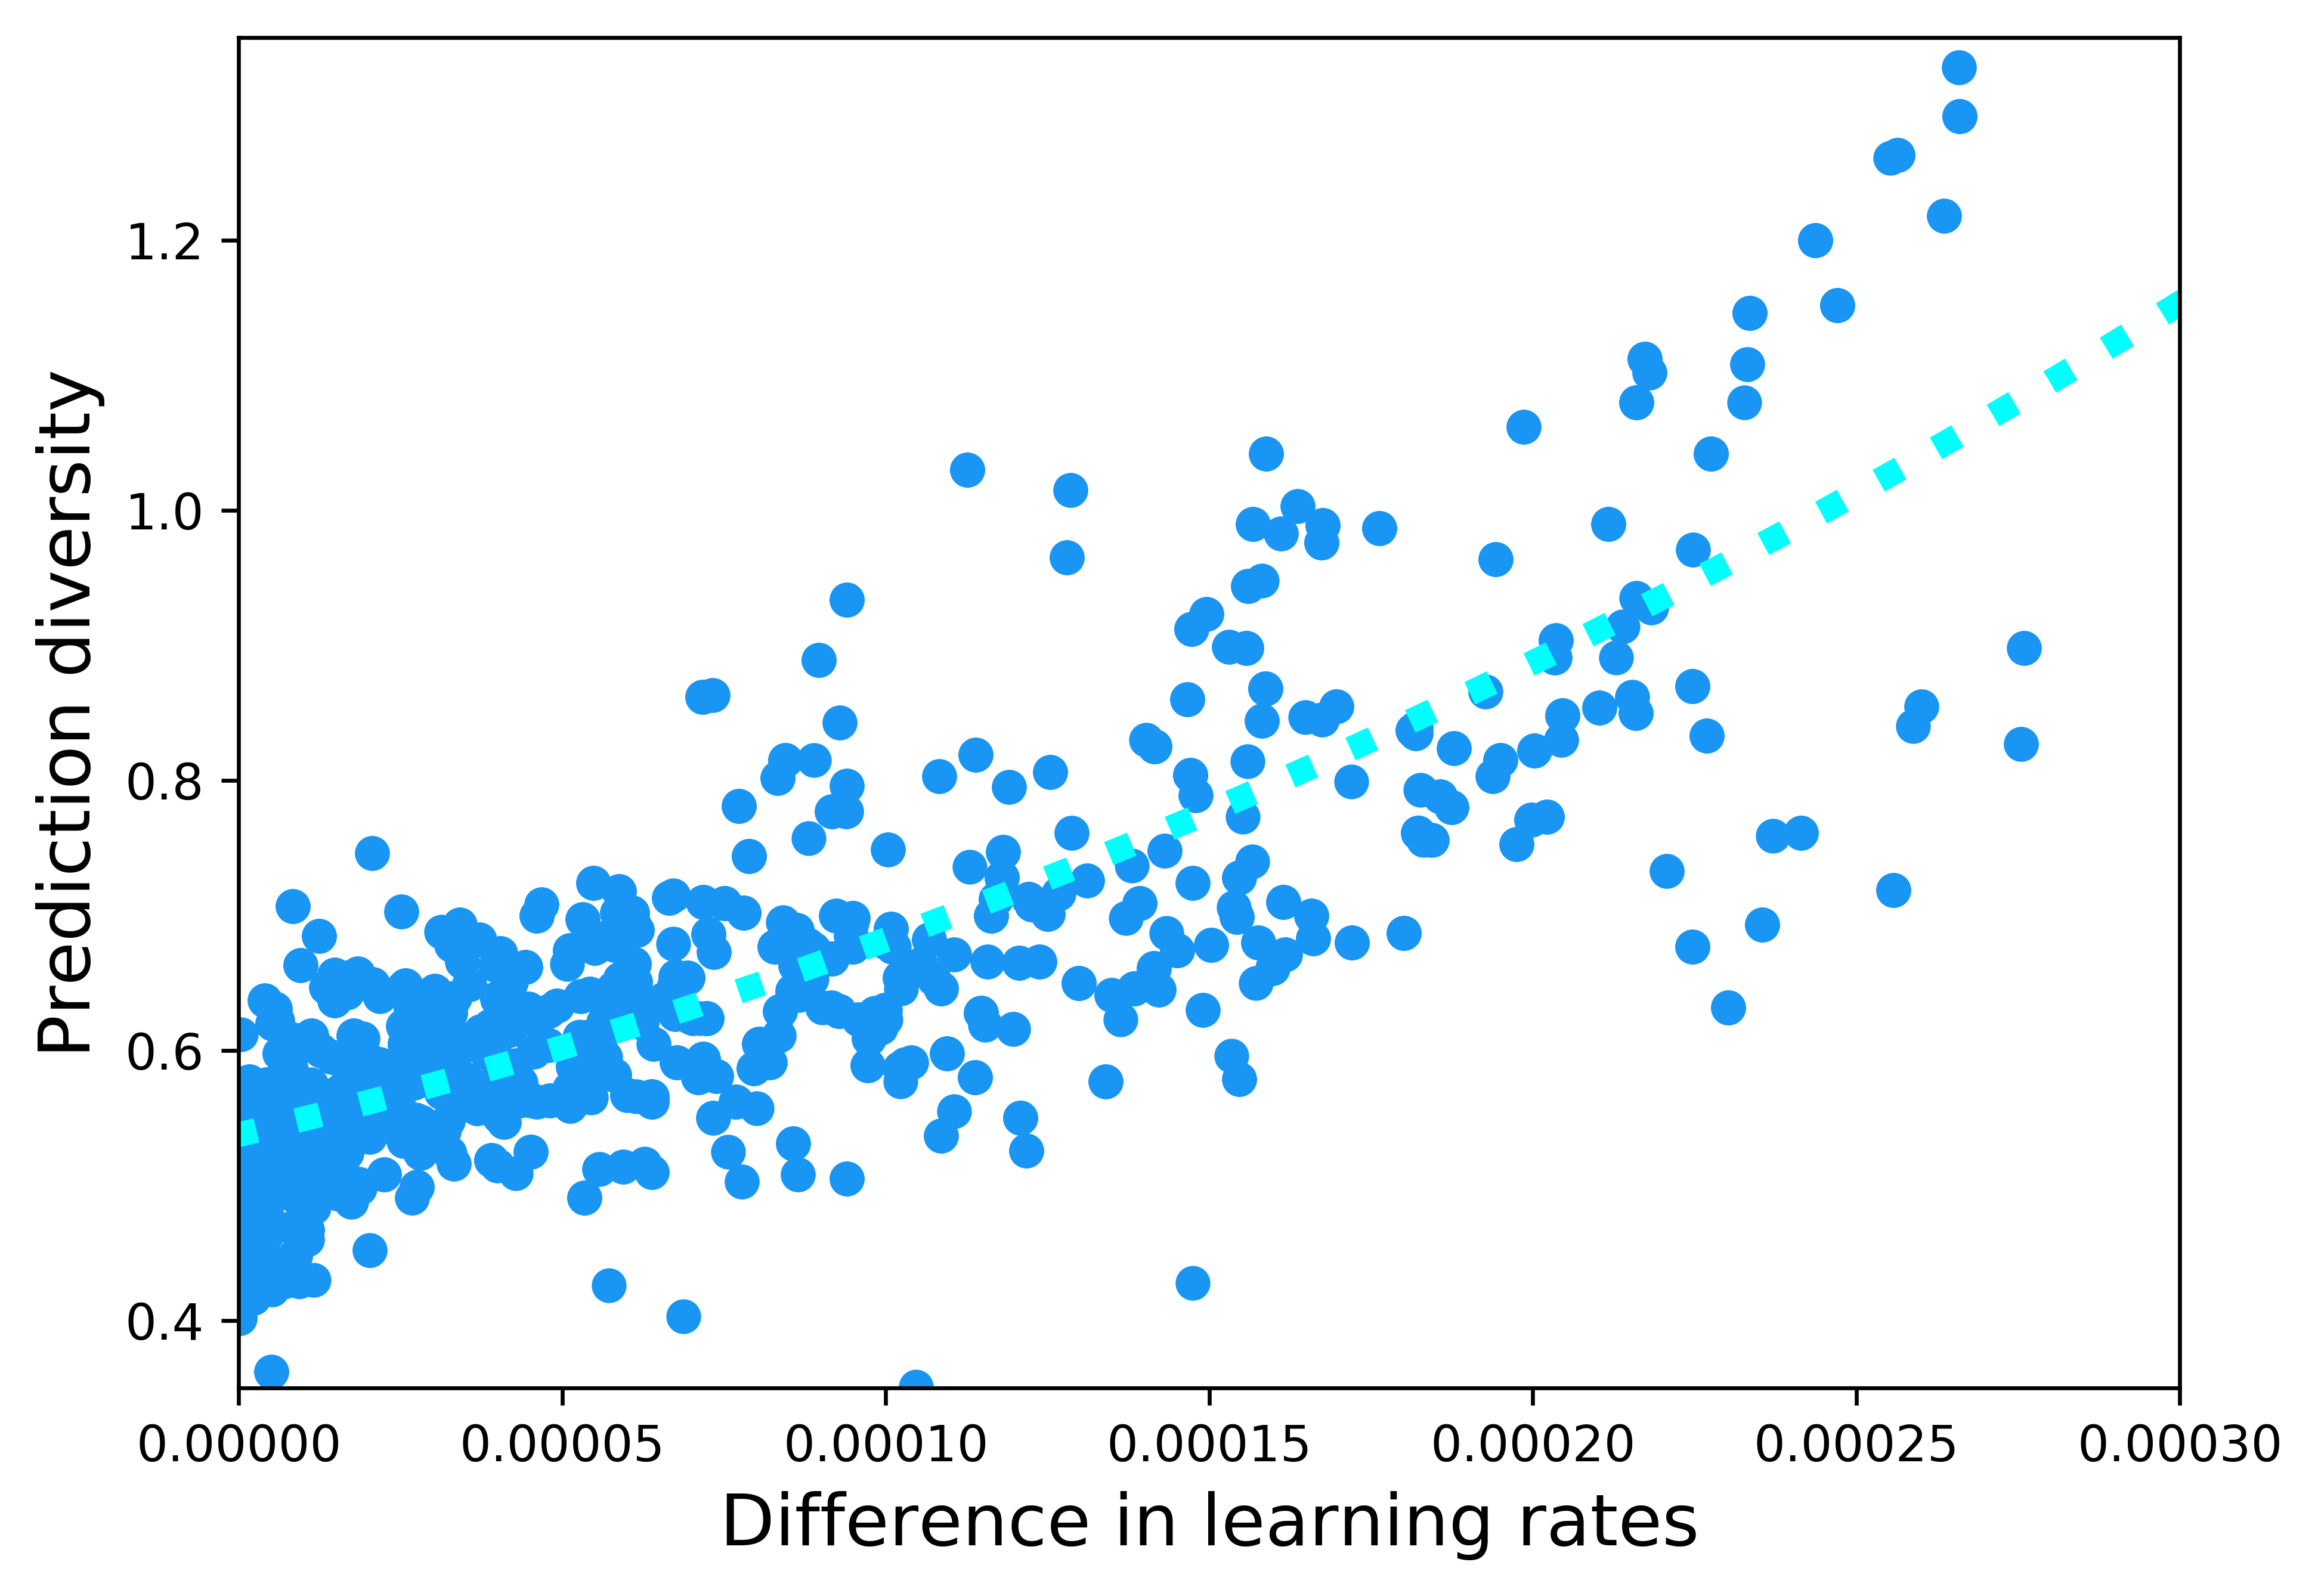
\includegraphics[width=1.0\textwidth]{pictures/files/final/diffruns_lrs_dr.png}%
        \caption{\reb{Prediction diversity ($\uparrow$) \cite{aksela2003comparison} between models.}}
        \label{fig:home0_lrs_dr}%
    \end{subfigure}%
    \begin{subfigure}{.5\textwidth}%
        \centering%
        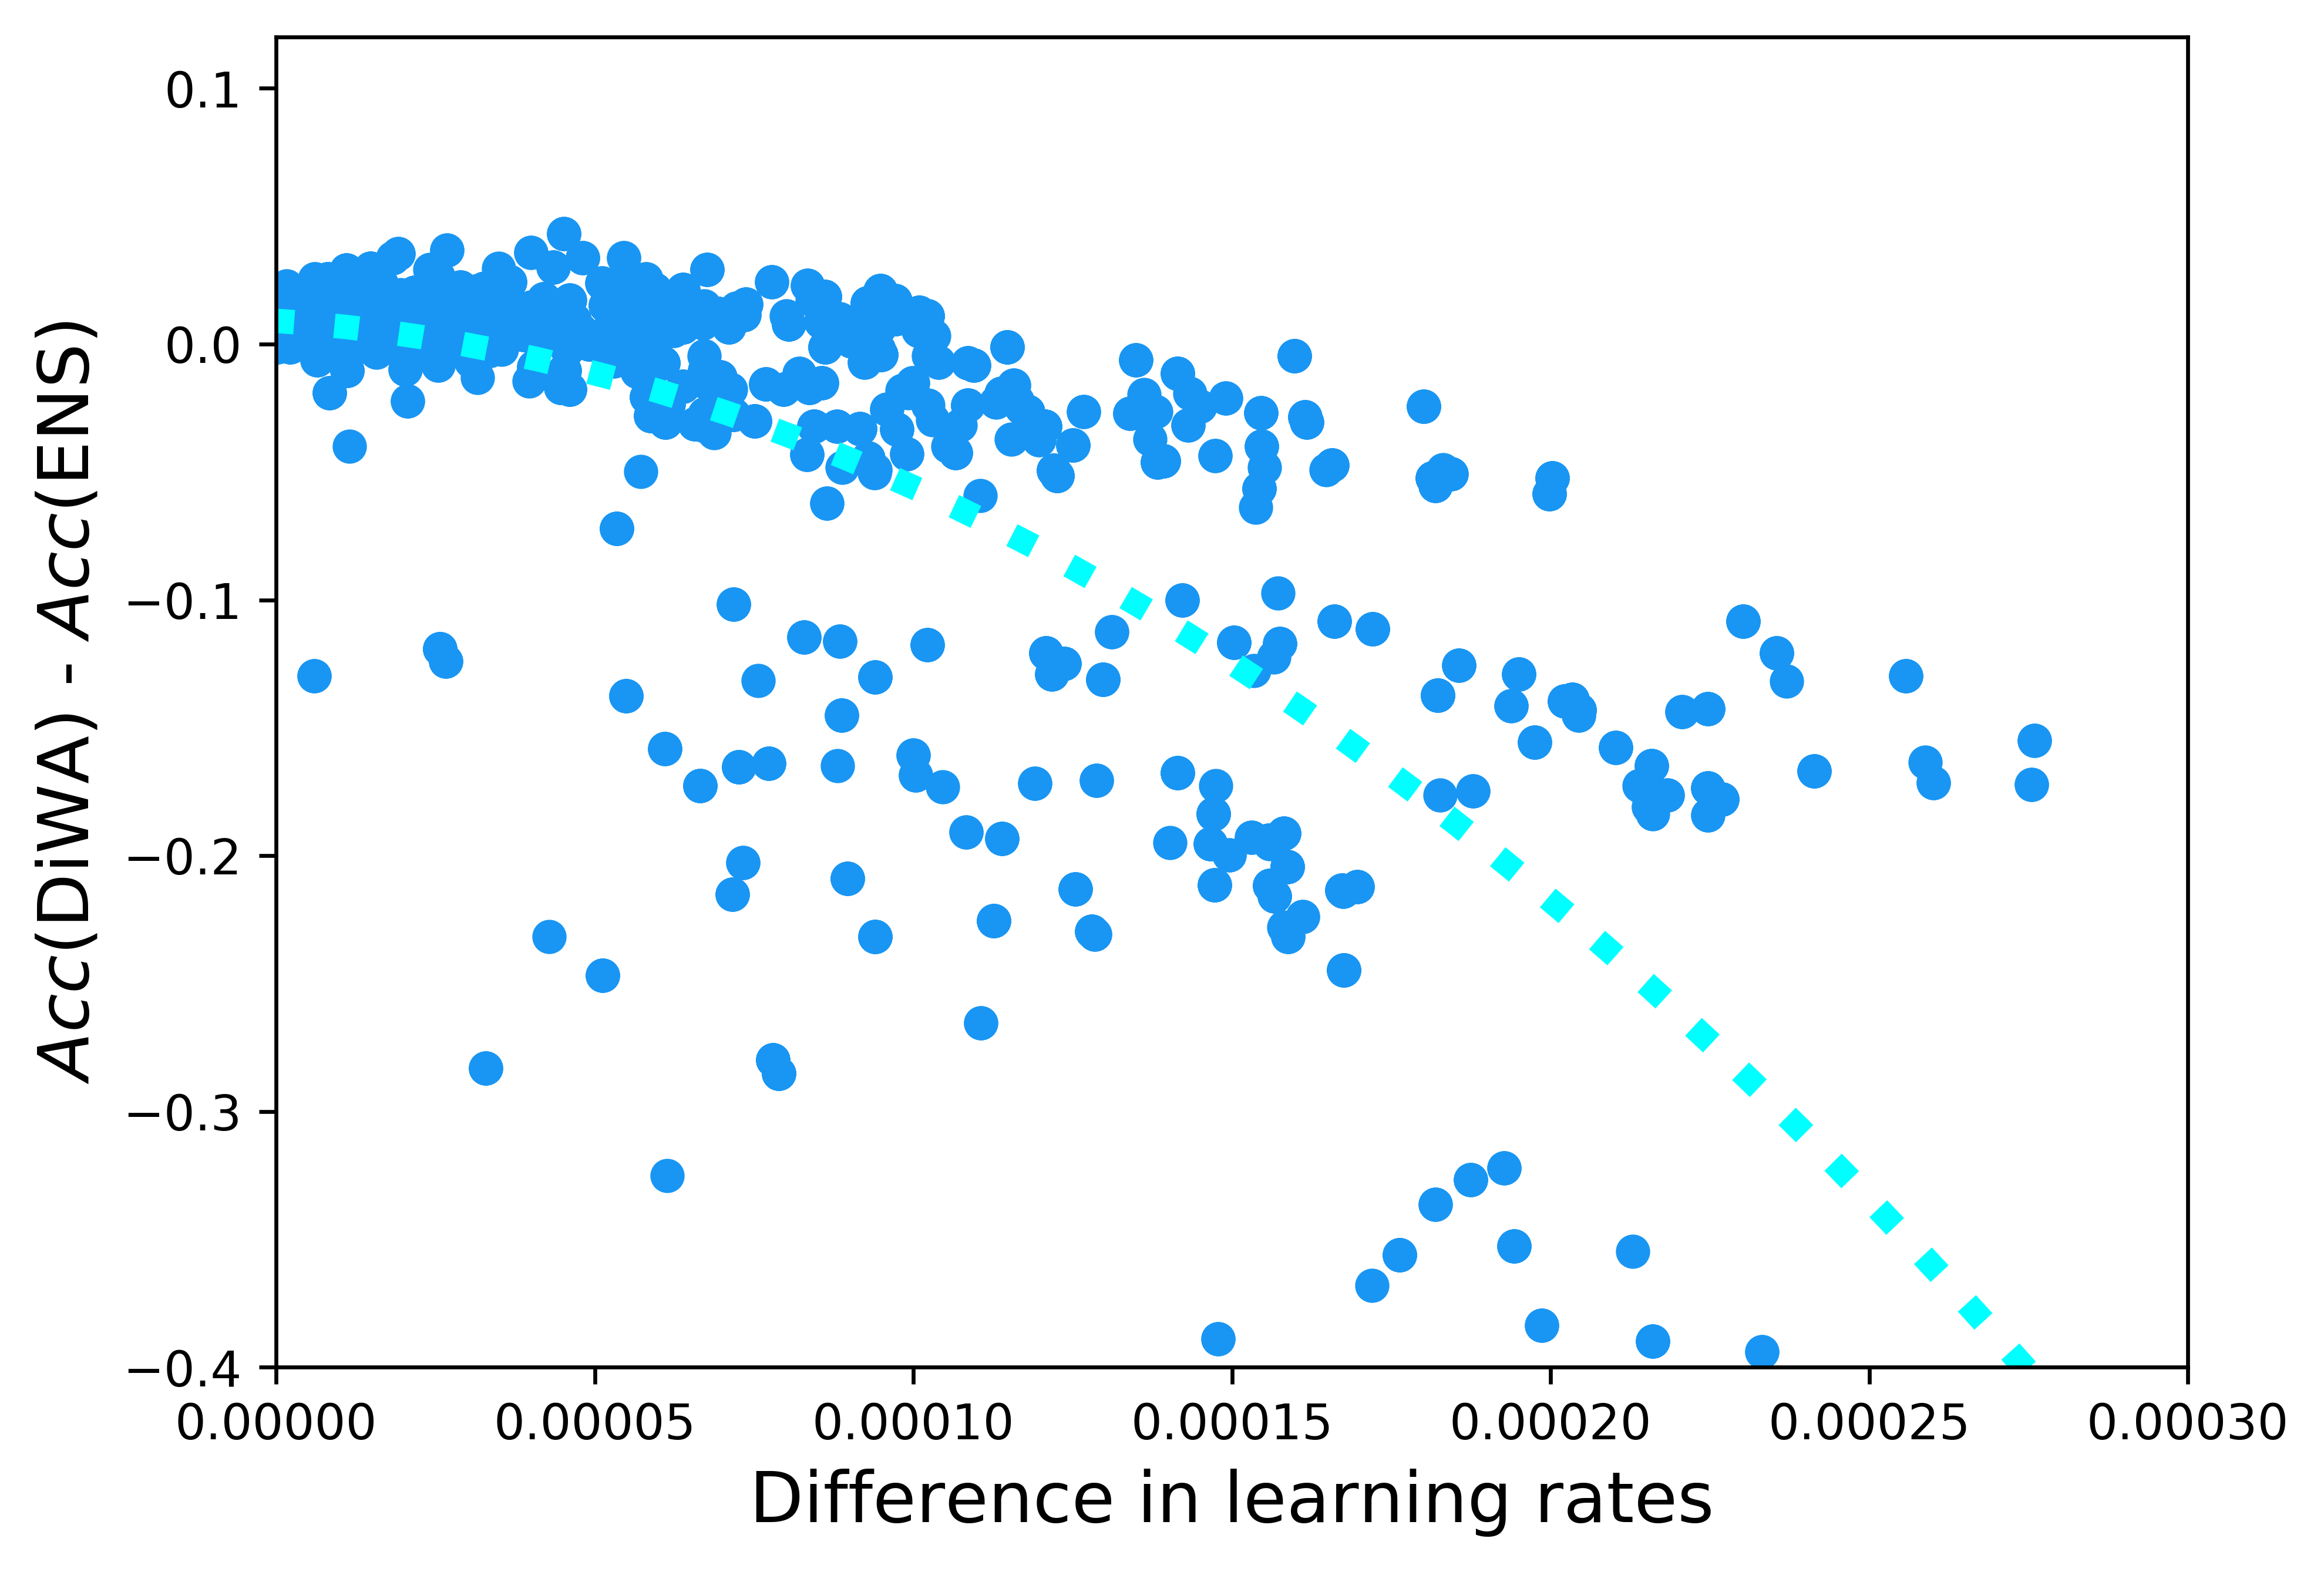
\includegraphics[width=1.0\textwidth]{pictures/files/final/diffruns_lrs_acc_net.png}%
        \caption{\reb{Accuracy ($\uparrow$) difference between DiWA and ENS.}}
        \label{fig:home0_lrs_acc}%
    \end{subfigure}%
    \caption{\reb{\textbf{Trade-off between diversity and averageability for various differences in learning rates}. Considering $M=2$ weights obtained from two learning procedures with learning rates $\text{lr}_1$ and $\text{lr}_2$ (sampled from the extreme distribution in \Cref{tab:hyperparam}), we plot in \Cref{fig:home0_lrs_dr} the prediction diversity for these $M=2$ models \versus $|\text{lr}_1-\text{lr}_2|$. Then, in \Cref{fig:home0_lrs_acc}, we plot the accuracy differences $\operatorname{Acc}(\text{DiWA})-\operatorname{Acc}(\text{ENS})$ \versus $|\text{lr}_1-\text{lr}_2|$.}}
    \label{fig:home0_lrs}%
\end{figure}%


\FloatBarrier
\subsection{On PACS}
\label{app:analysis_pacs}
We perform in \Cref{fig:soup:pacs_div_soup-netm} on domain \enquote{Art} from PACS the same core diversity-based experiments than on OfficeHome in \Cref{sect:analysis}.
We recover the same conclusions.
\begin{figure}[h]%
    \centering%
    \begin{subfigure}{.33\textwidth}%
        \centering%
        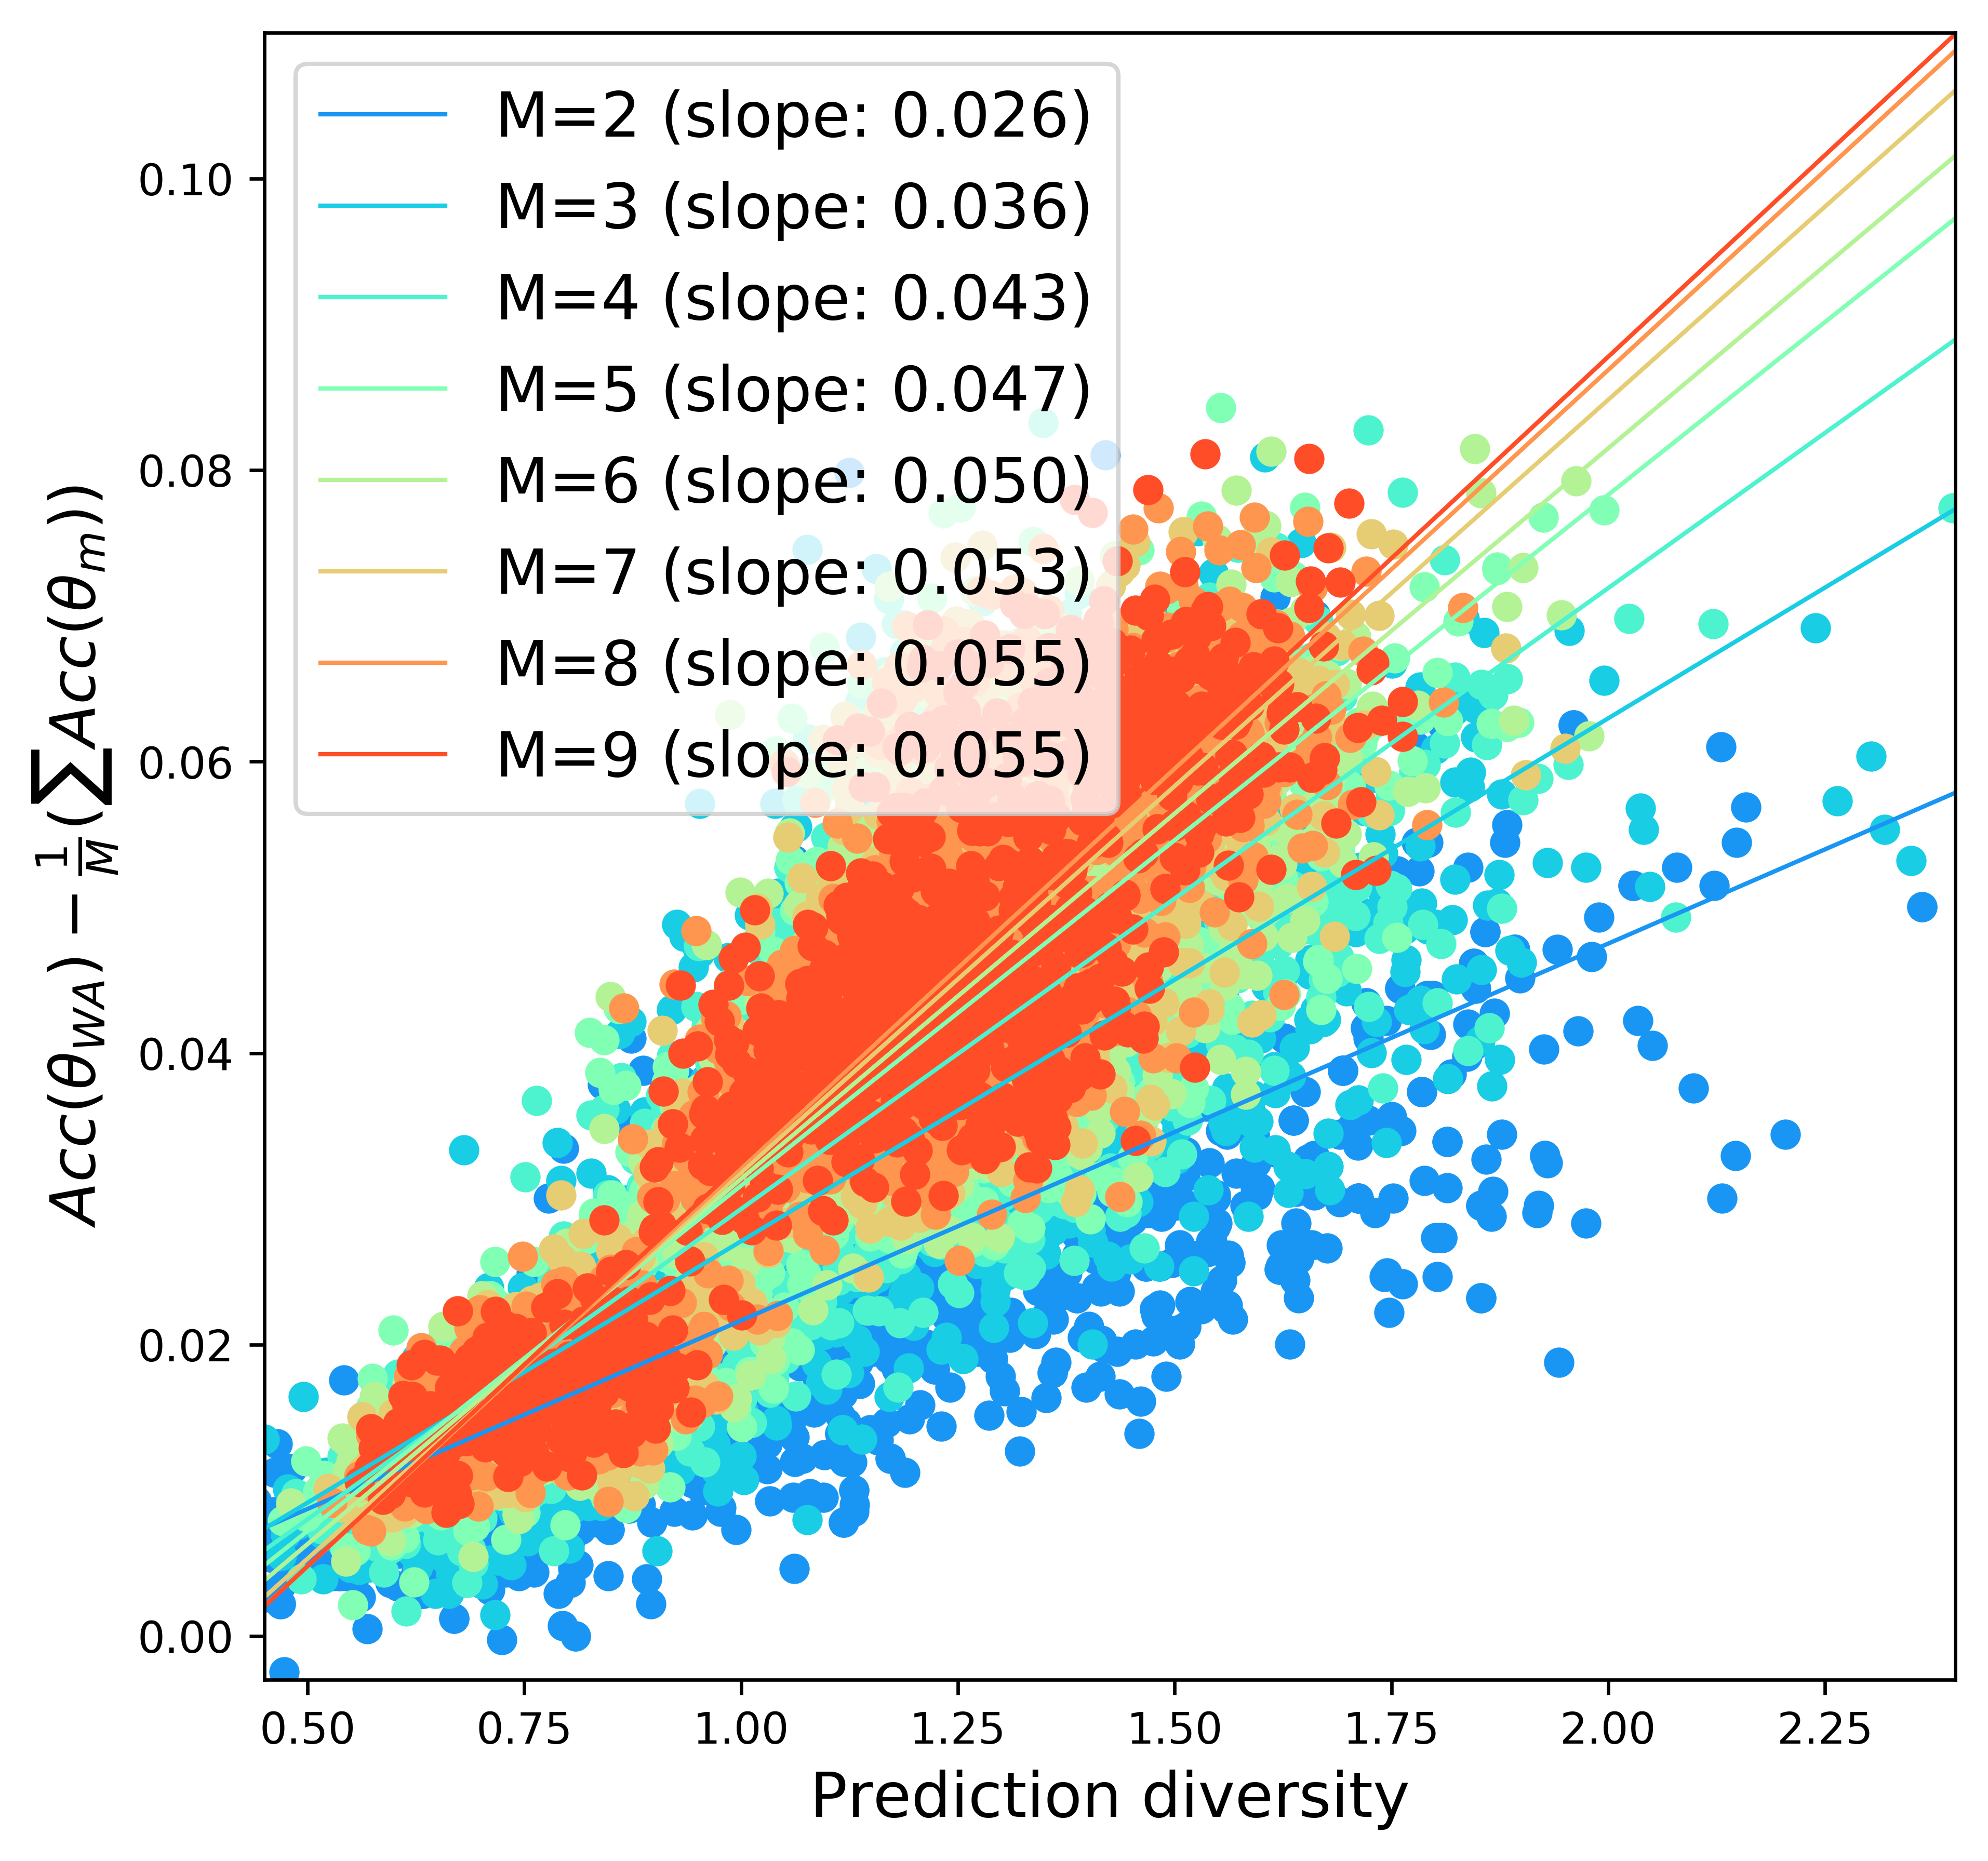
\includegraphics[width=\linewidth]{pictures/files/final/pacs0_samediffruns_dr_soup-netm.png}%
        \caption{Same as \Cref{fig:home0_dr_soup-netm}.}%
        \label{fig:pacs_dr_soup-netm}%
    \end{subfigure}%
    \begin{subfigure}{.33\textwidth}%
        \centering%
        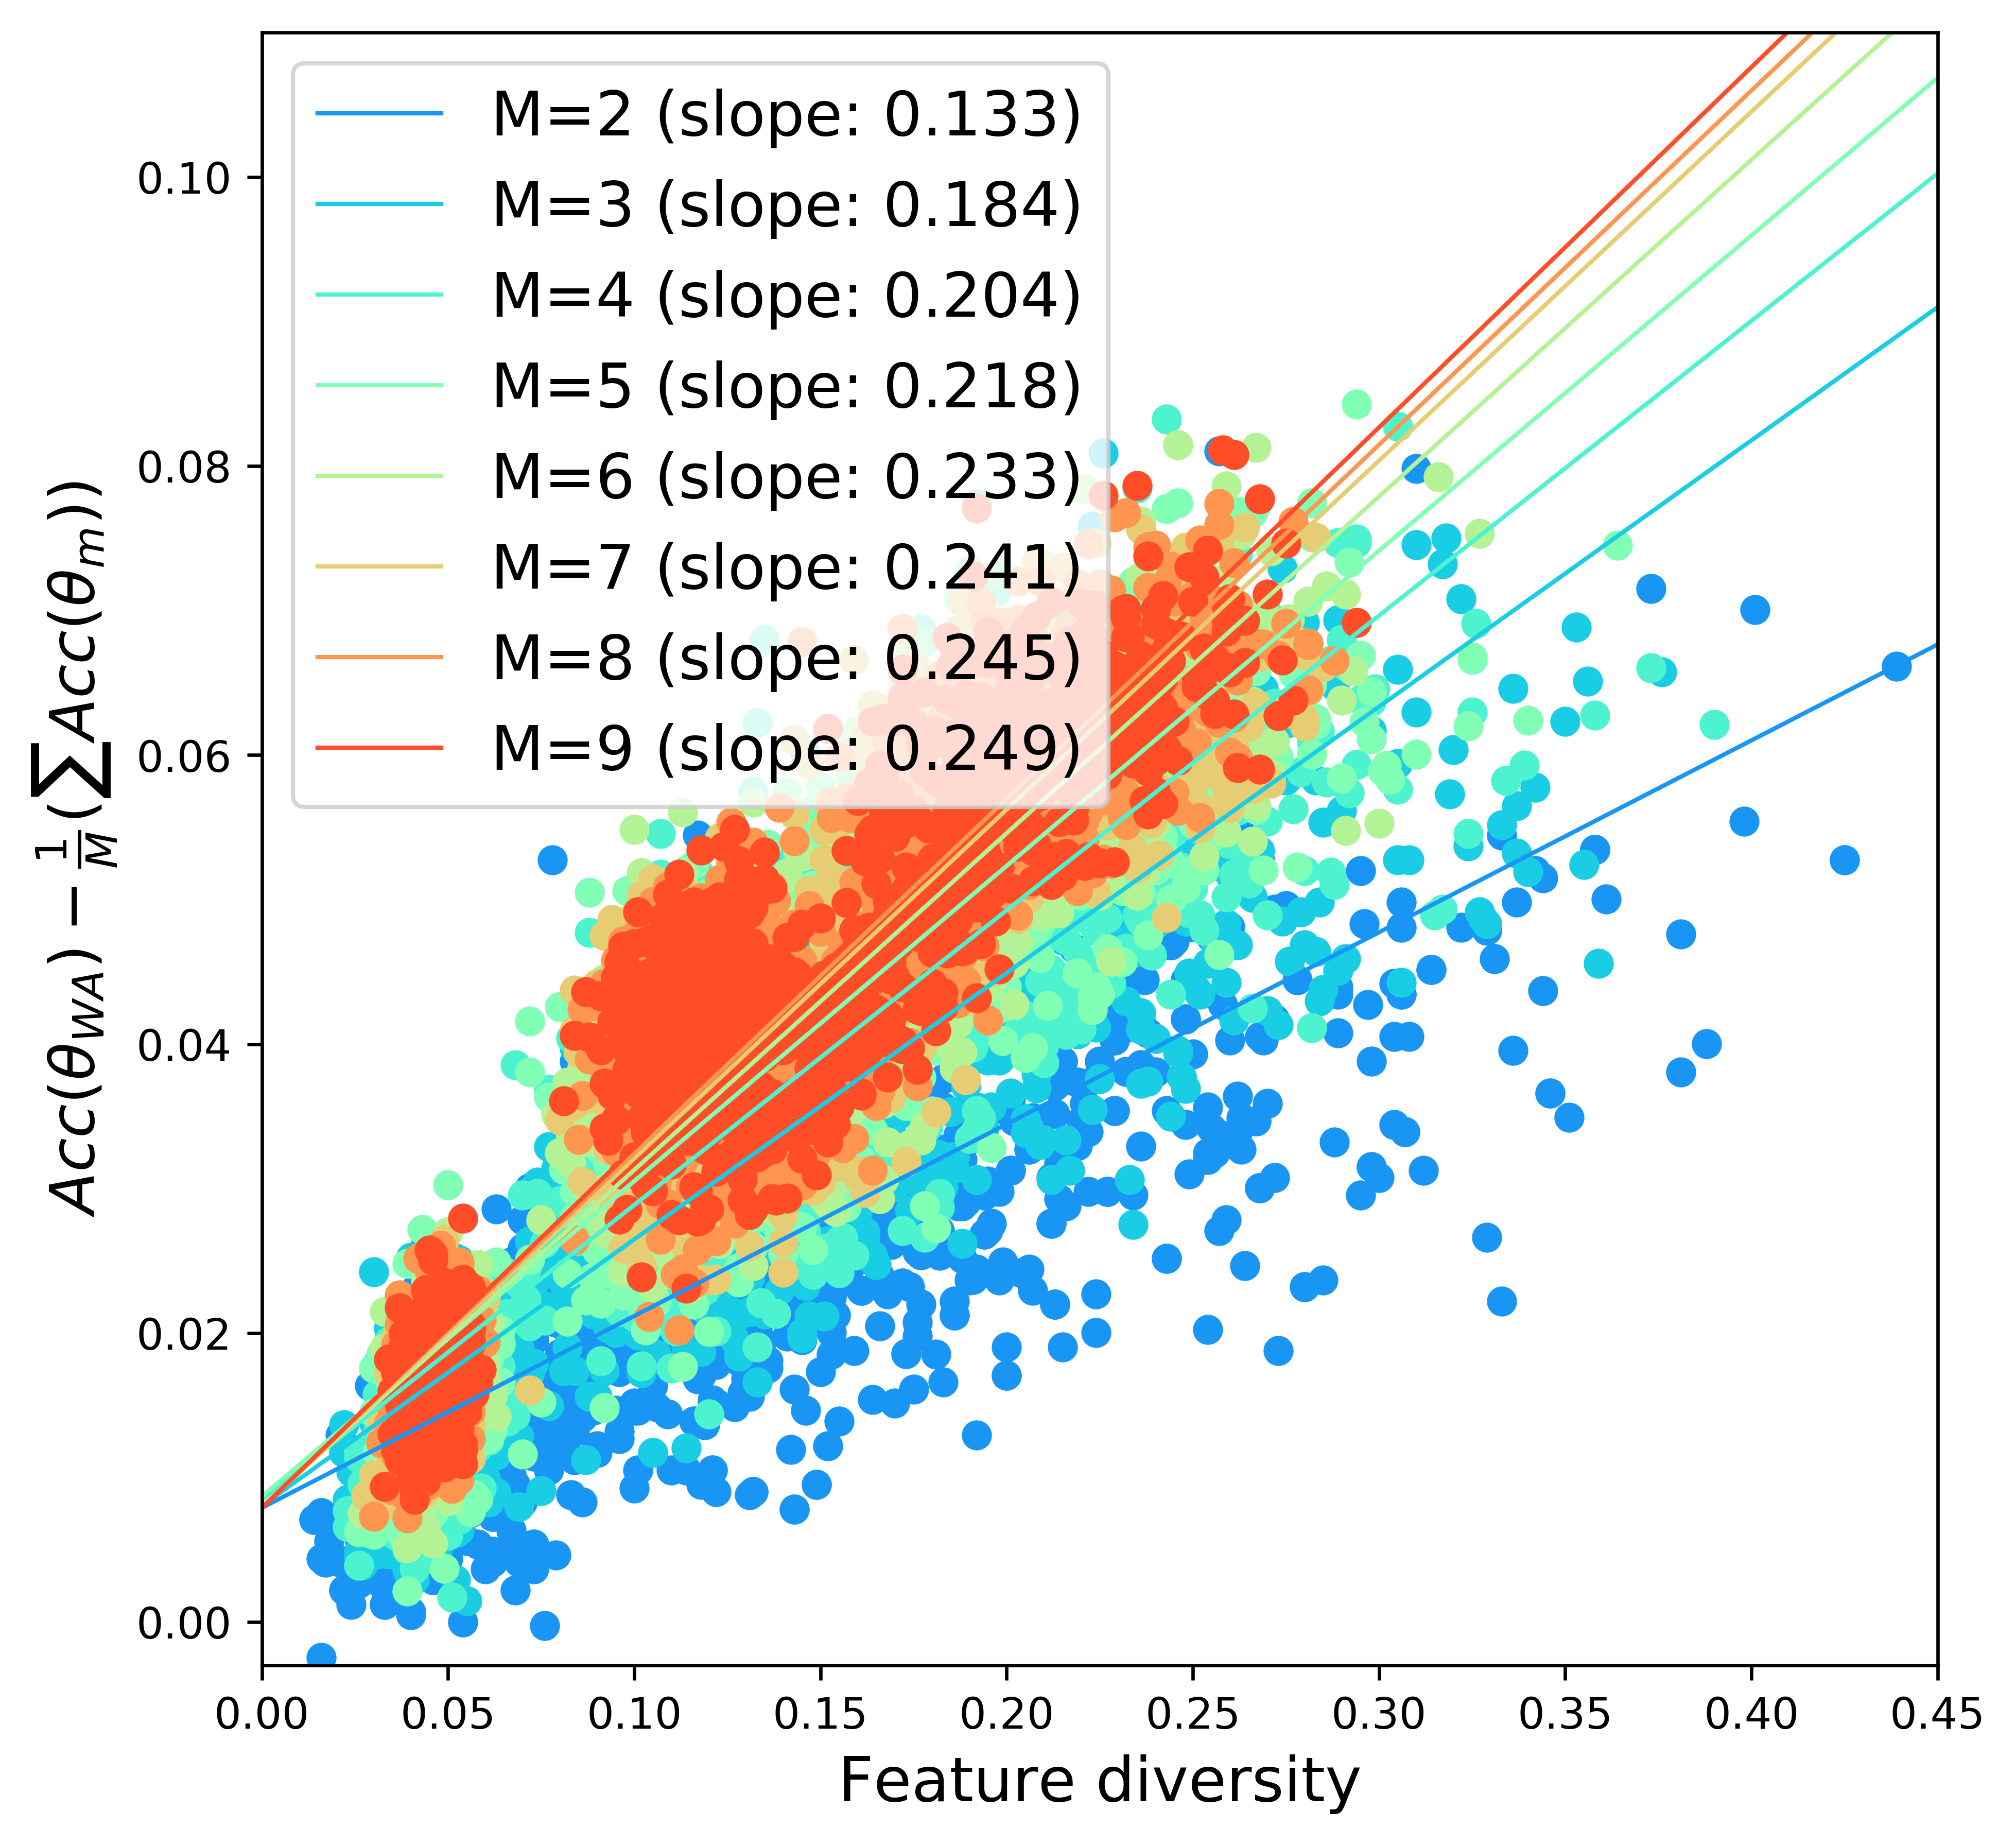
\includegraphics[width=\linewidth]{pictures/files/final/pacs0_samediffruns_df_soup-netm.png}%
        \caption{Same as \Cref{fig:home0_df_soup-netm}.}%
        \label{fig:pacs_df_soup-netm}%
    \end{subfigure}%
    \begin{subfigure}{.33\textwidth}%
        \centering%
        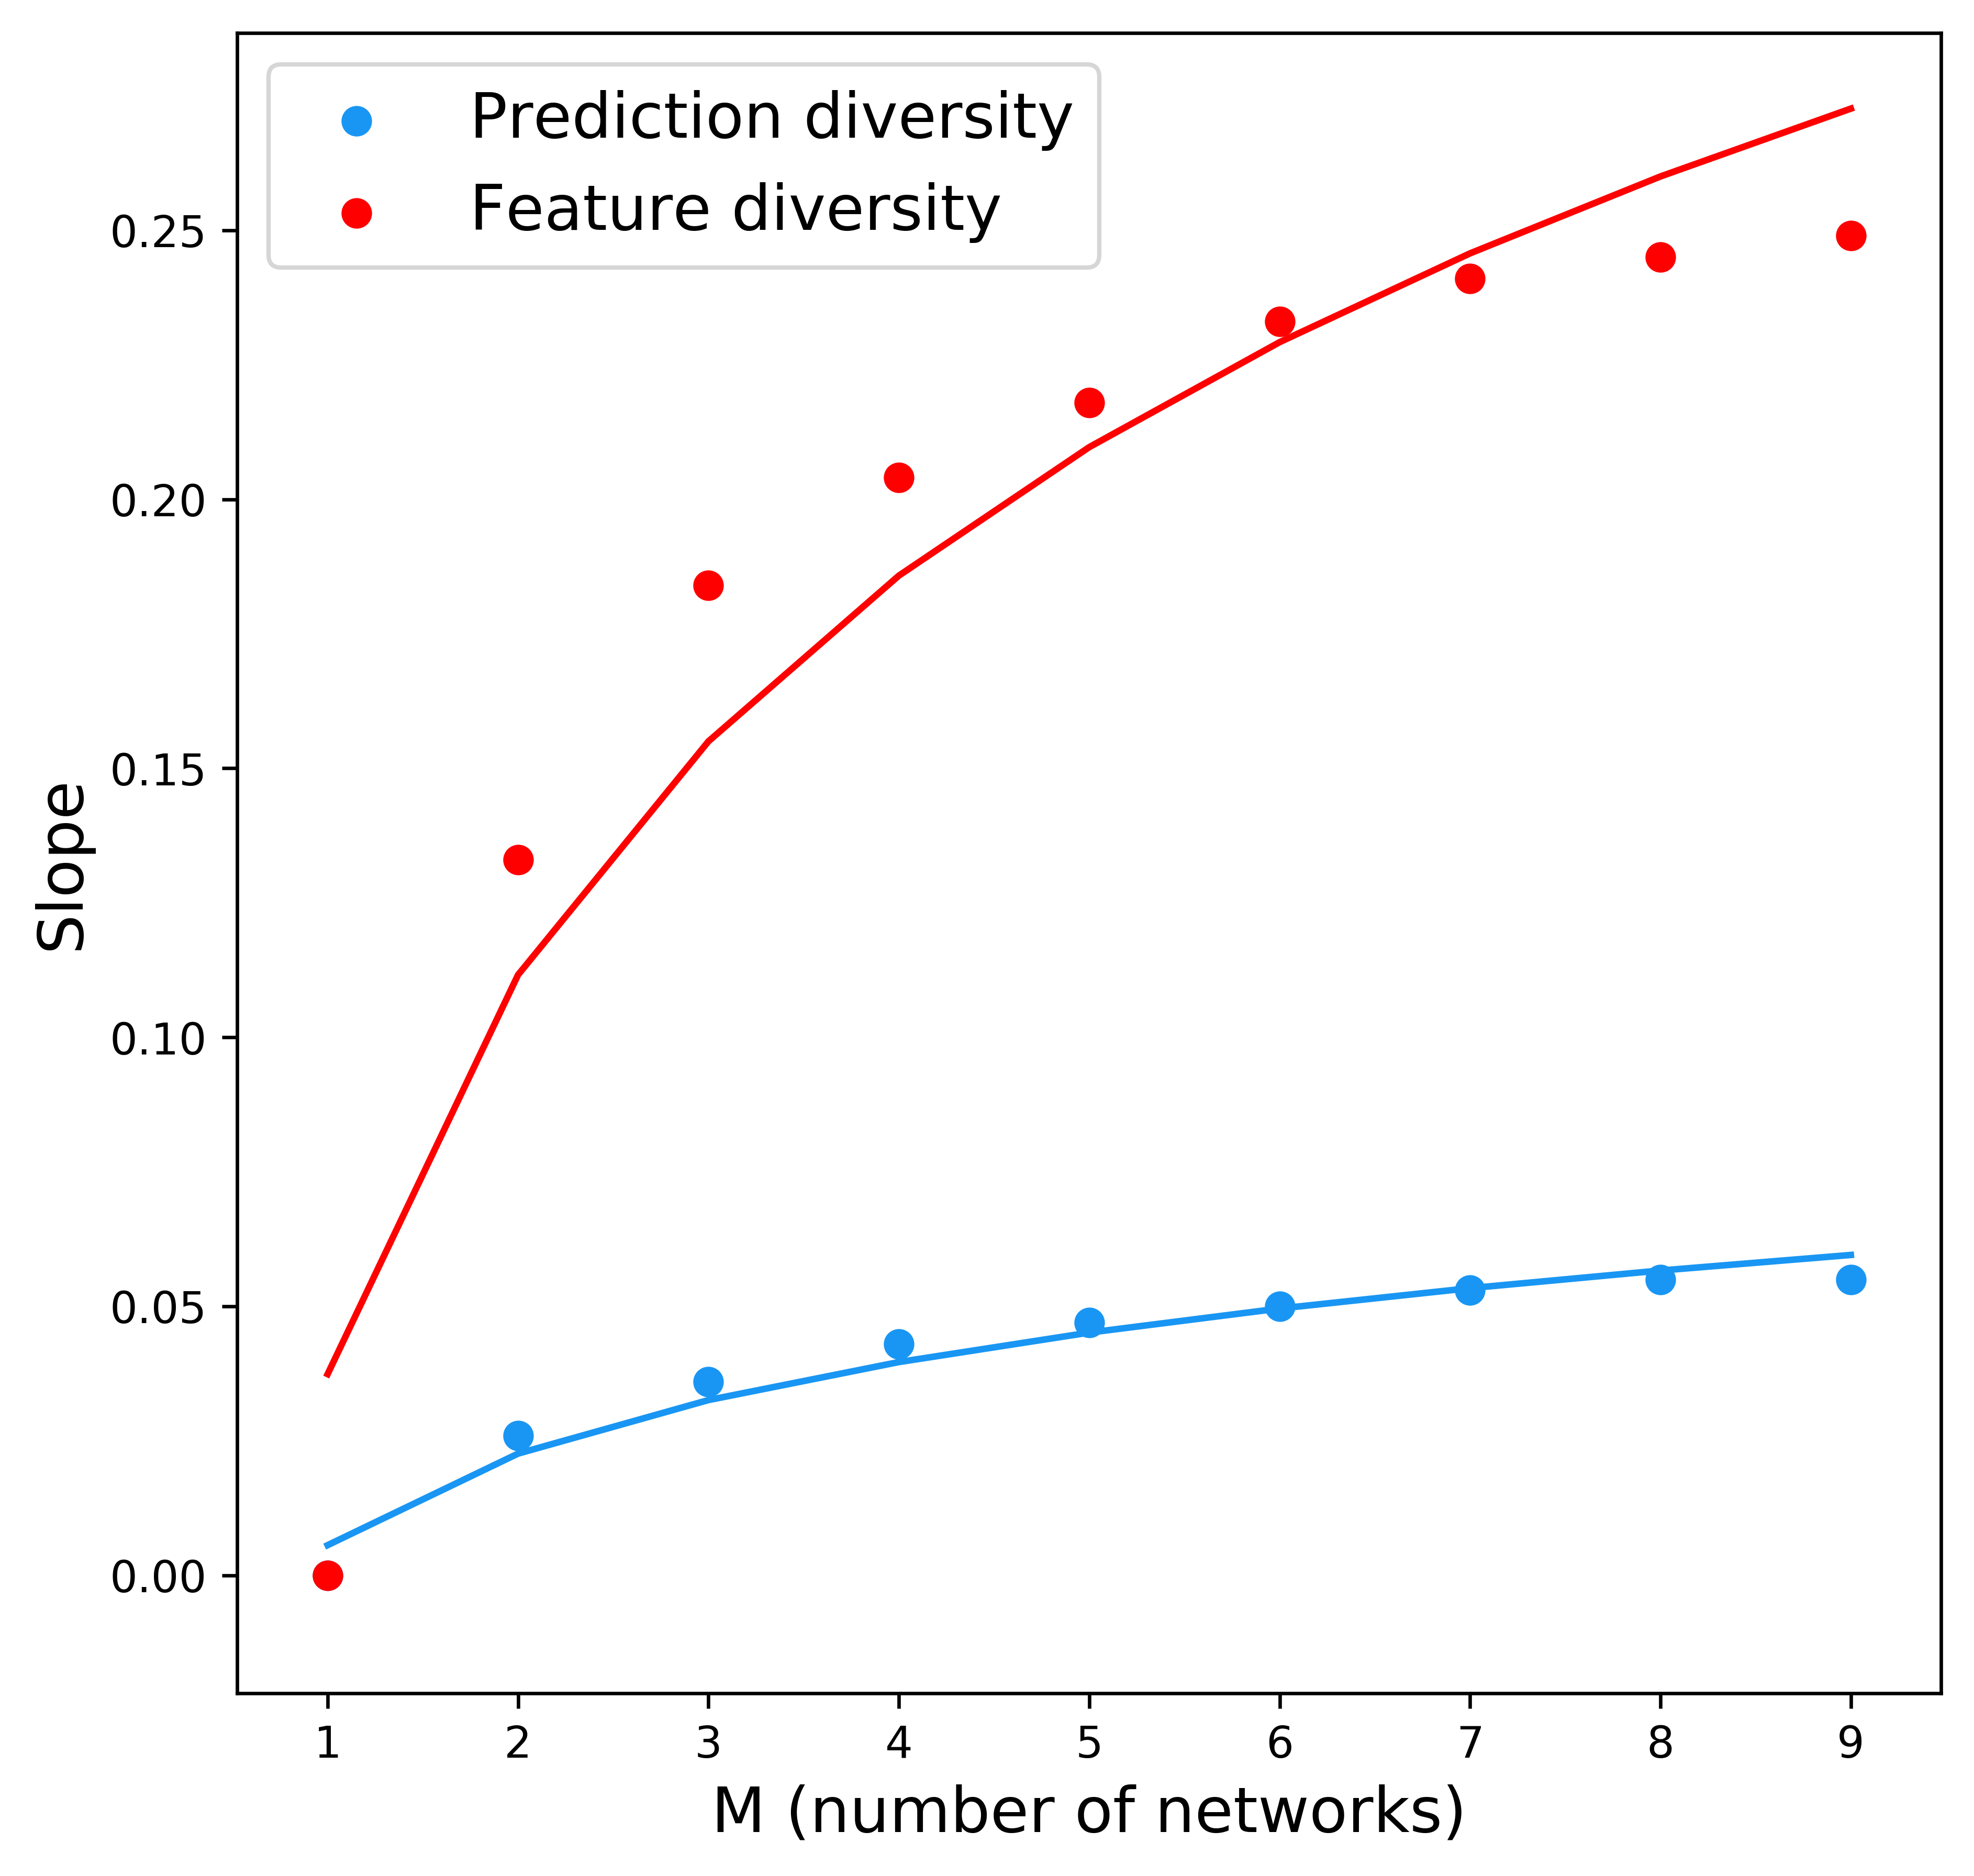
\includegraphics[width=\textwidth]{pictures/files/final/pacs0_m_slope.png}%
        \caption{Same as \Cref{fig:soup:m_slope}.}
        \label{fig:soup:pacs_m_slope}%
    \end{subfigure}%
    \caption{Same analysis on PACS as previously done on OfficeHome.}%
    \label{fig:soup:pacs_div_soup-netm}%
\end{figure}%

\begin{figure}[H]
    \vspace{-1.em}
    \centering
    \begin{subfigure}{.33\textwidth}%
        \centering%
        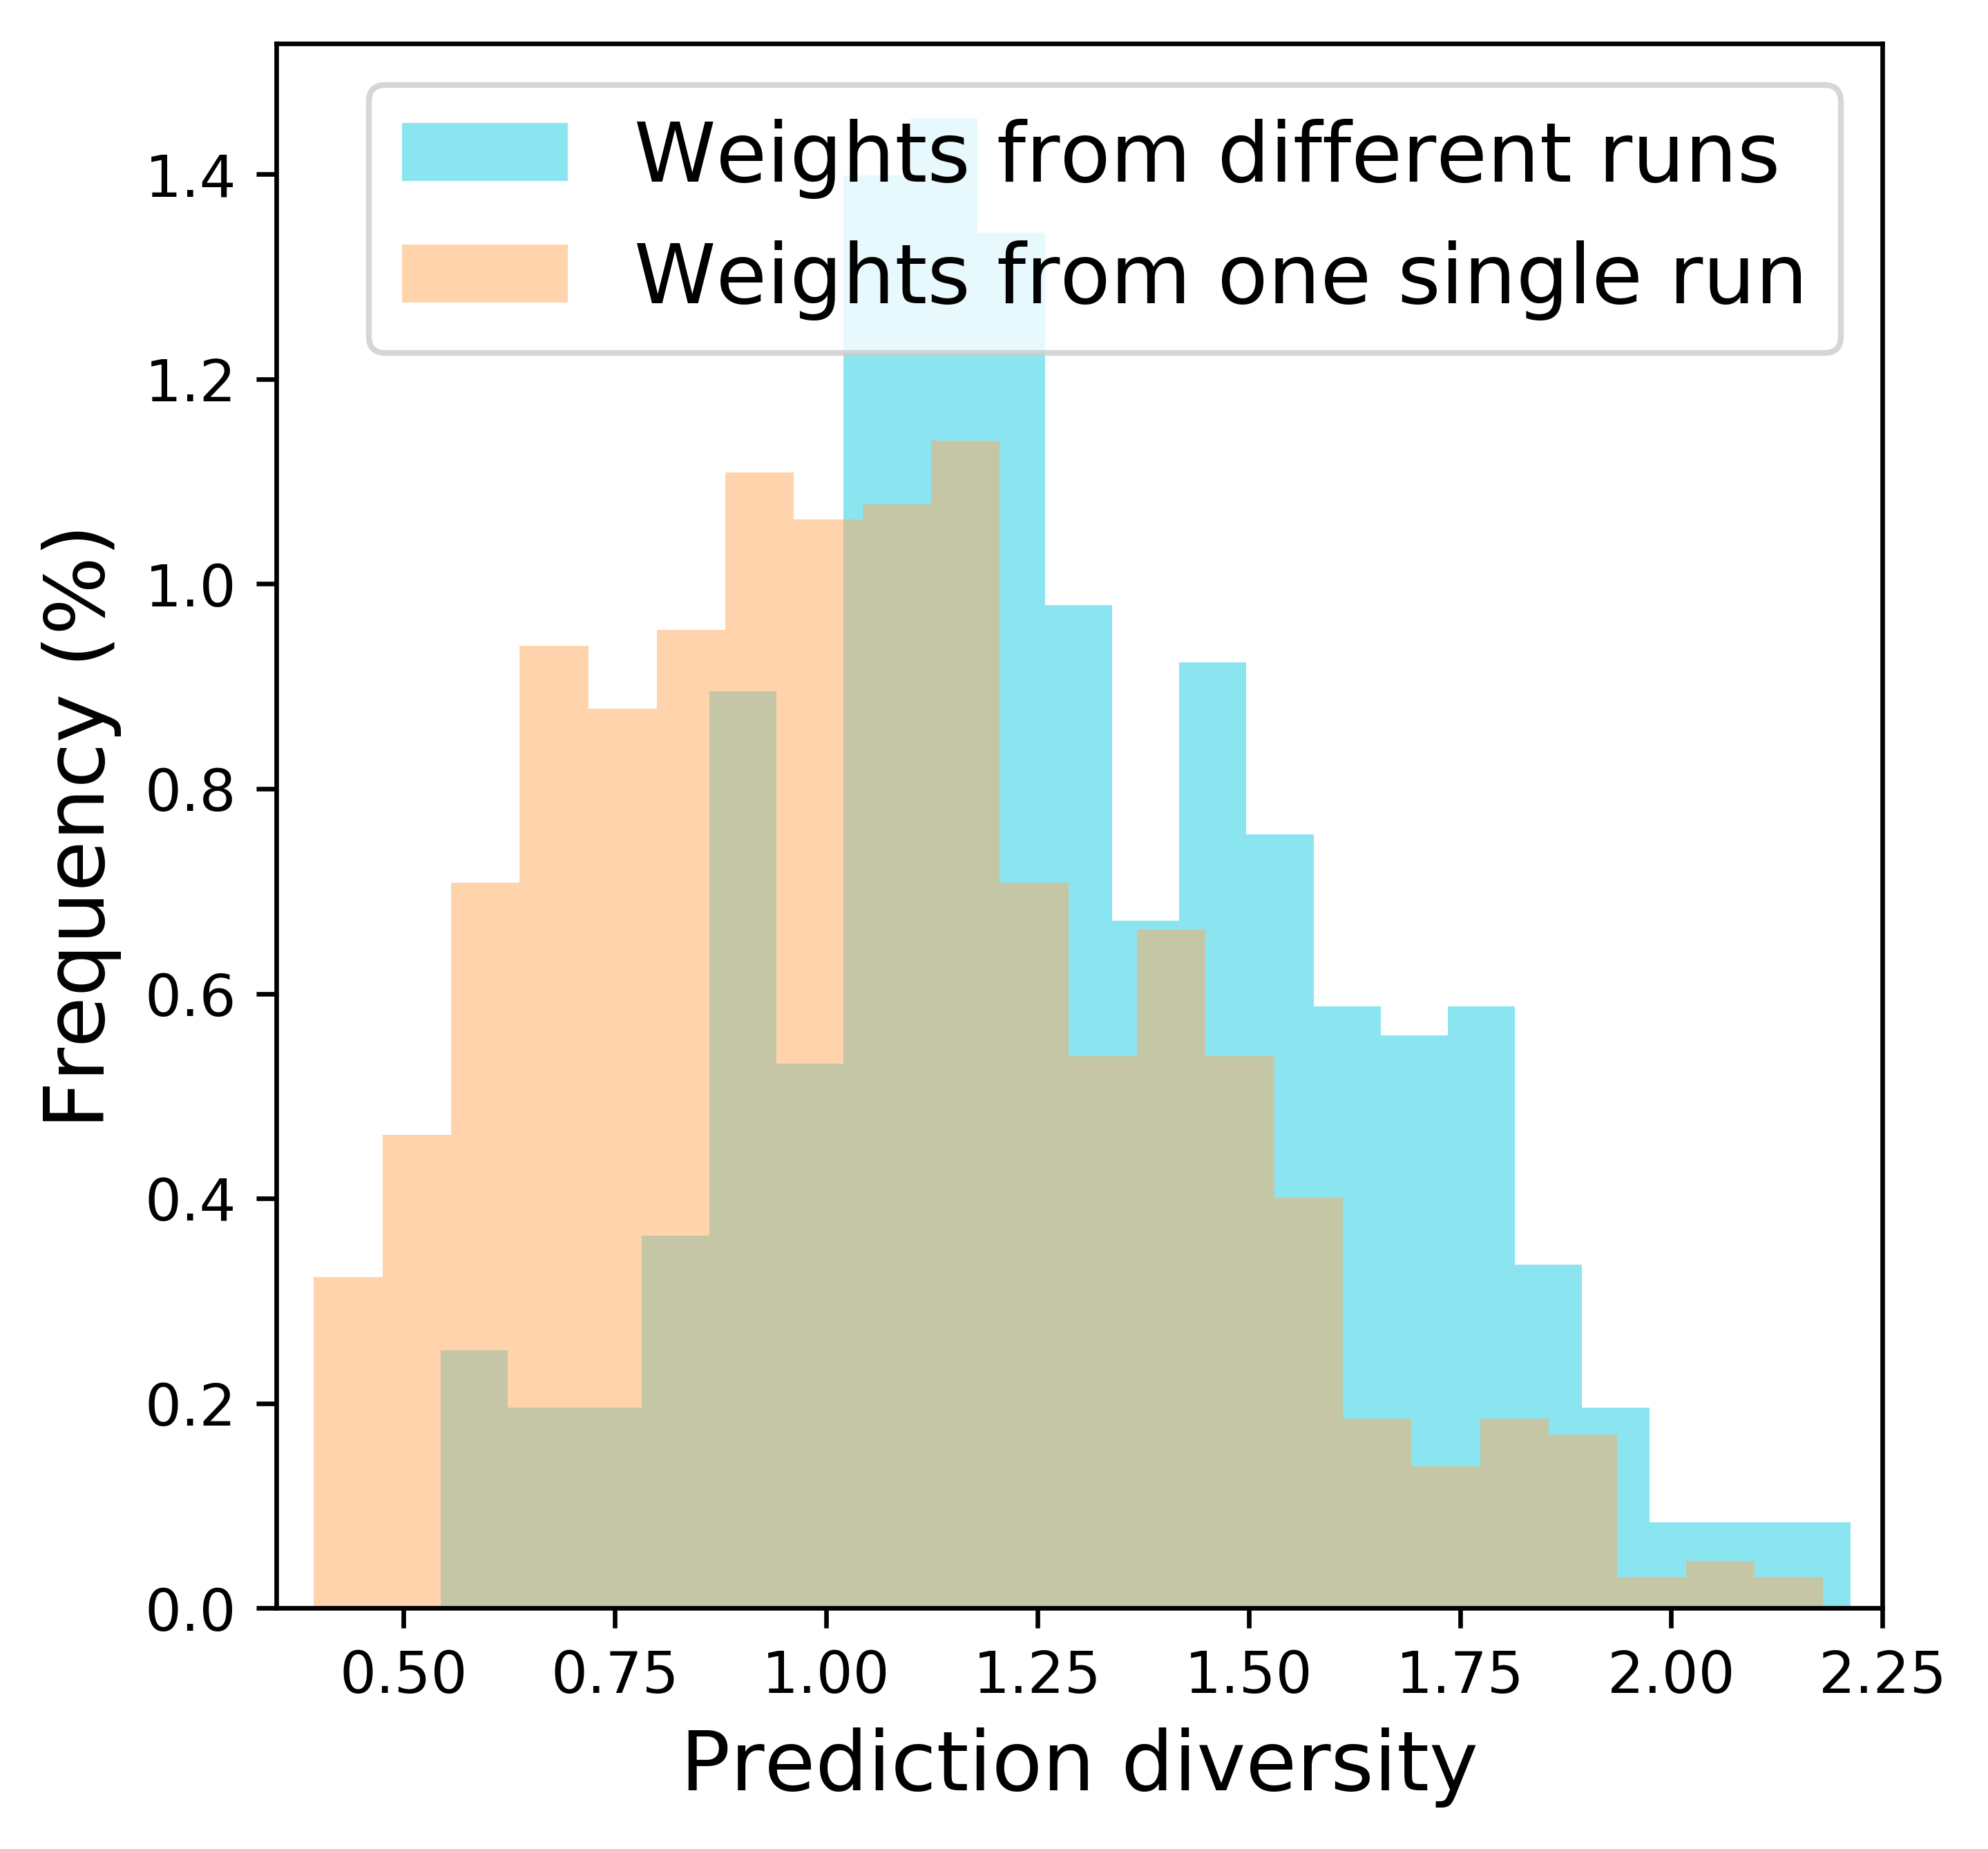
\includegraphics[width=\textwidth]{pictures/files/final/pacs0_hist_dr.png}%
        \caption{Same as \Cref{fig:home0_dr_frequency}.}
    \end{subfigure}%
    \begin{subfigure}{.33\textwidth}%
        \centering%
        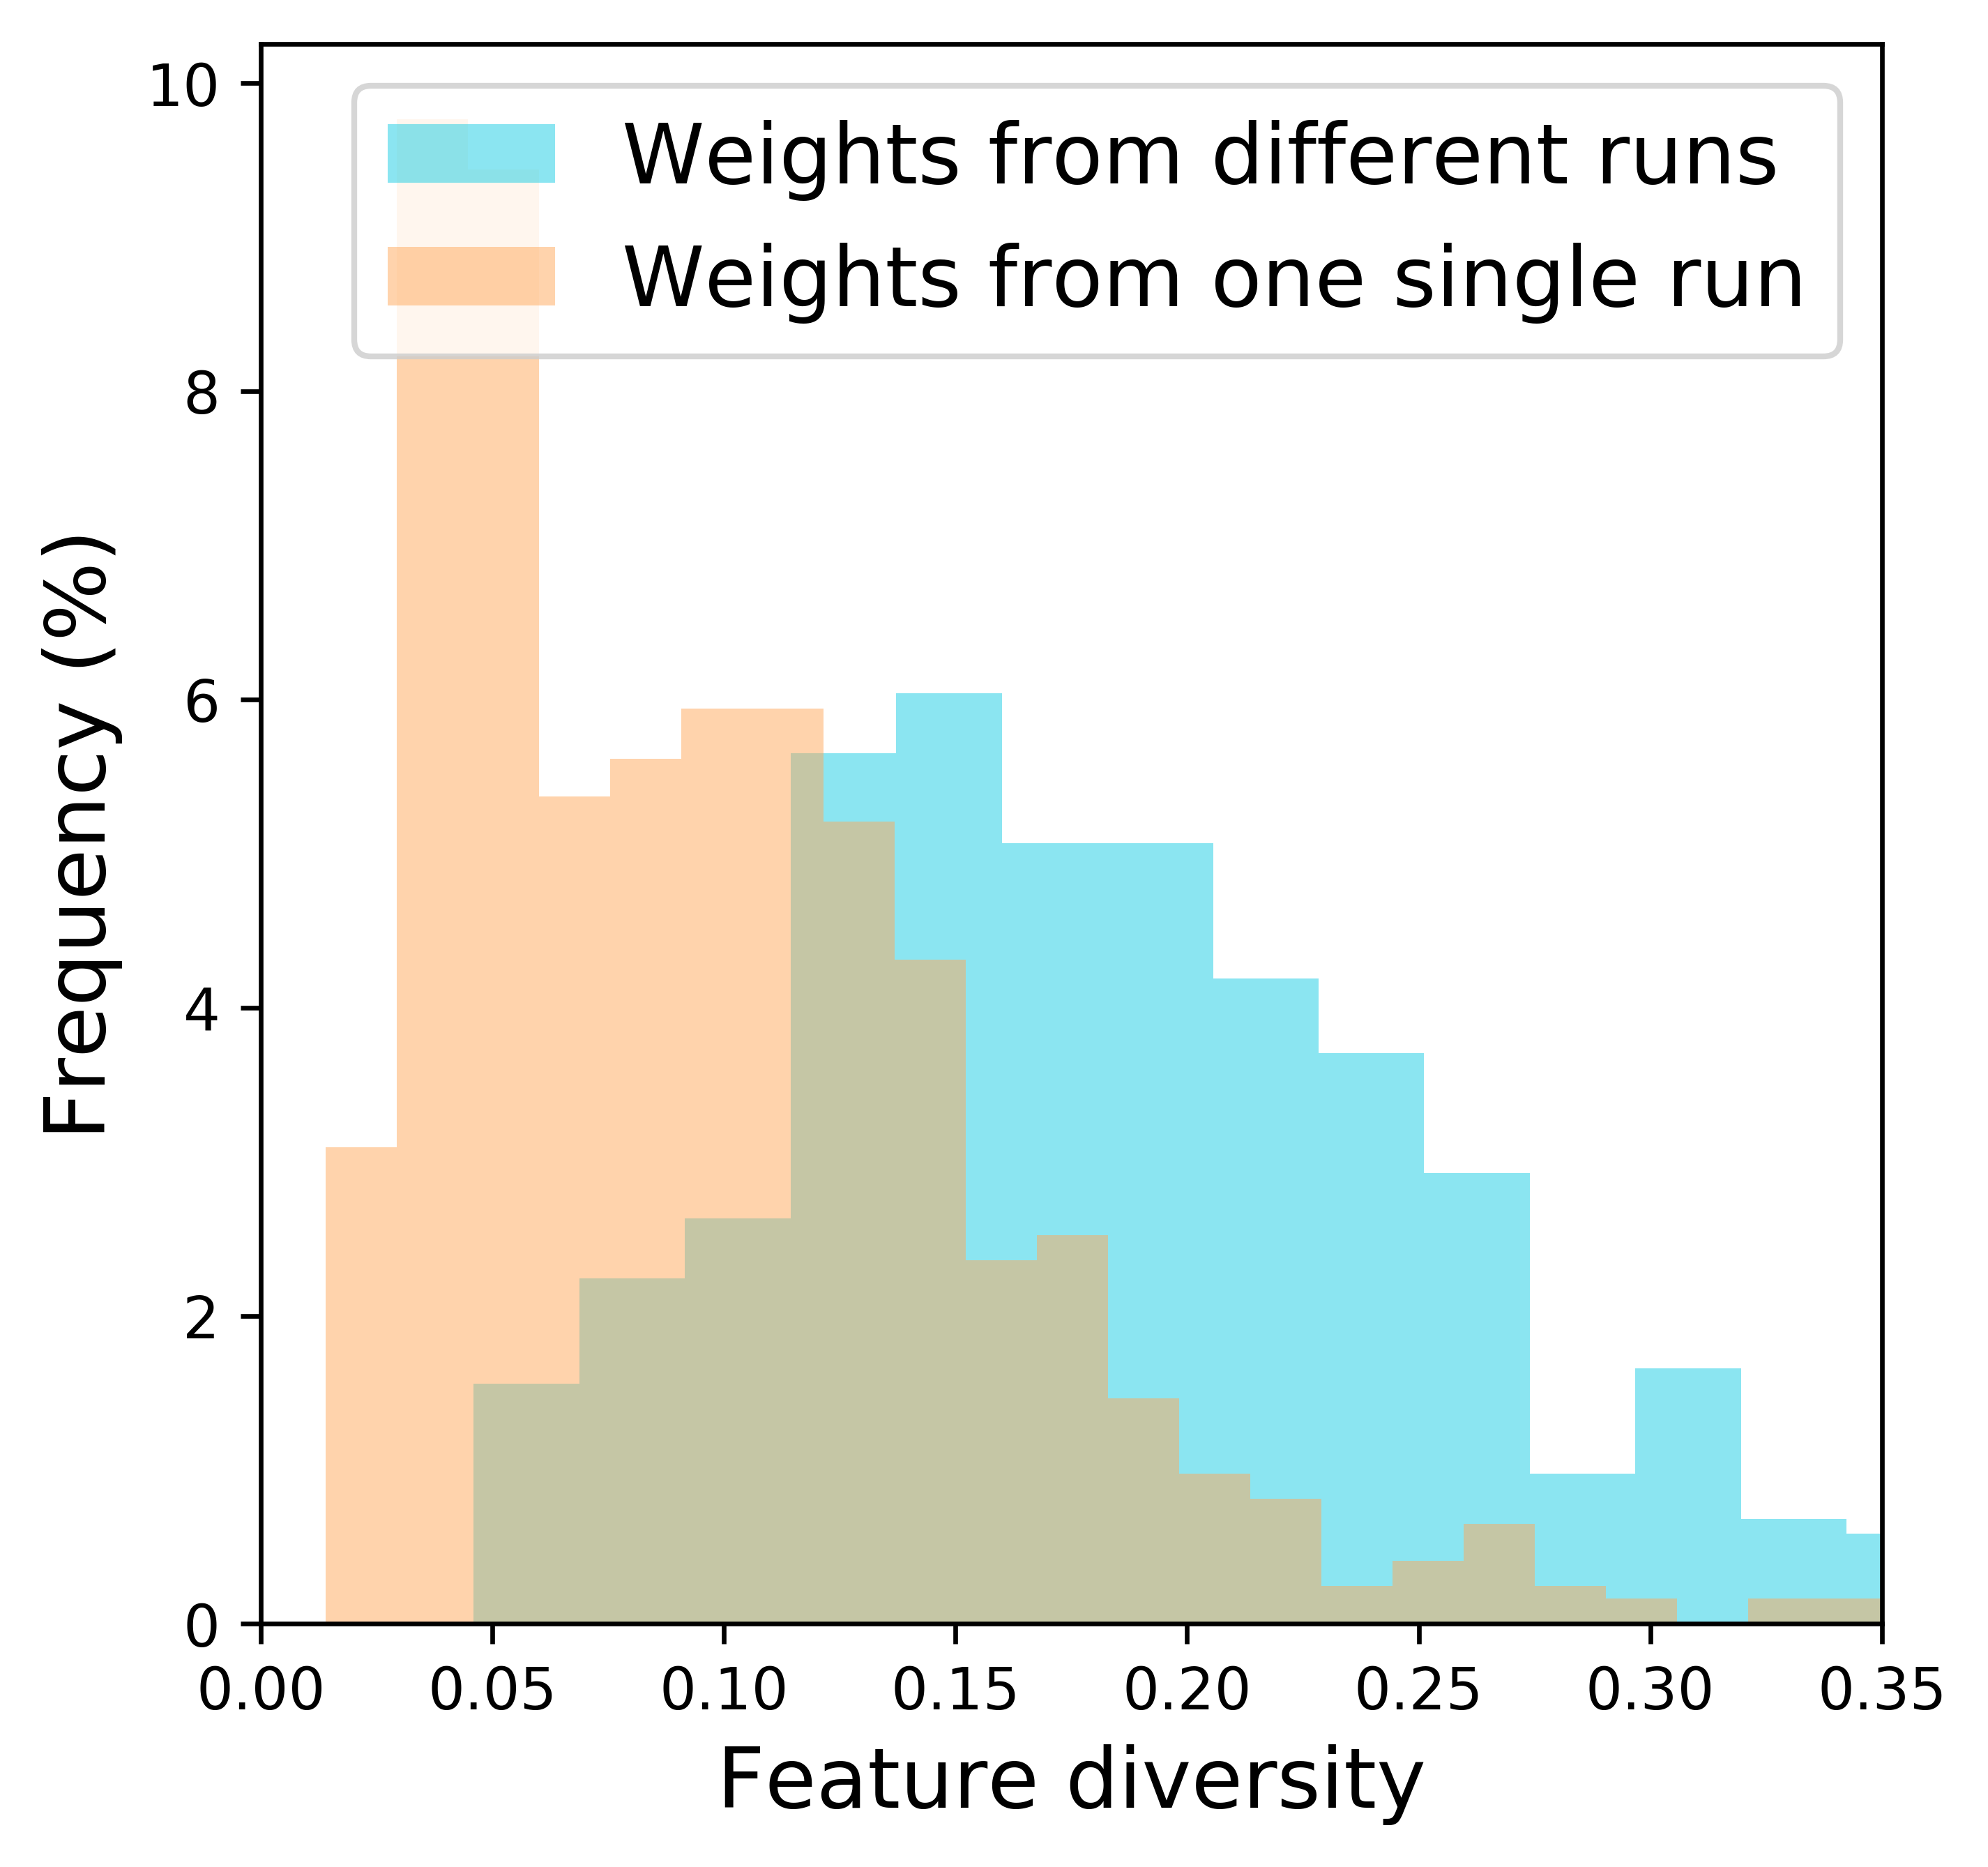
\includegraphics[width=\textwidth]{pictures/files/final/pacs0_hist_df.png}%
        \caption{Same as \Cref{fig:home0_df_frequency}.}
    \end{subfigure}%
    \begin{subfigure}{.33\textwidth}%
        \centering%
        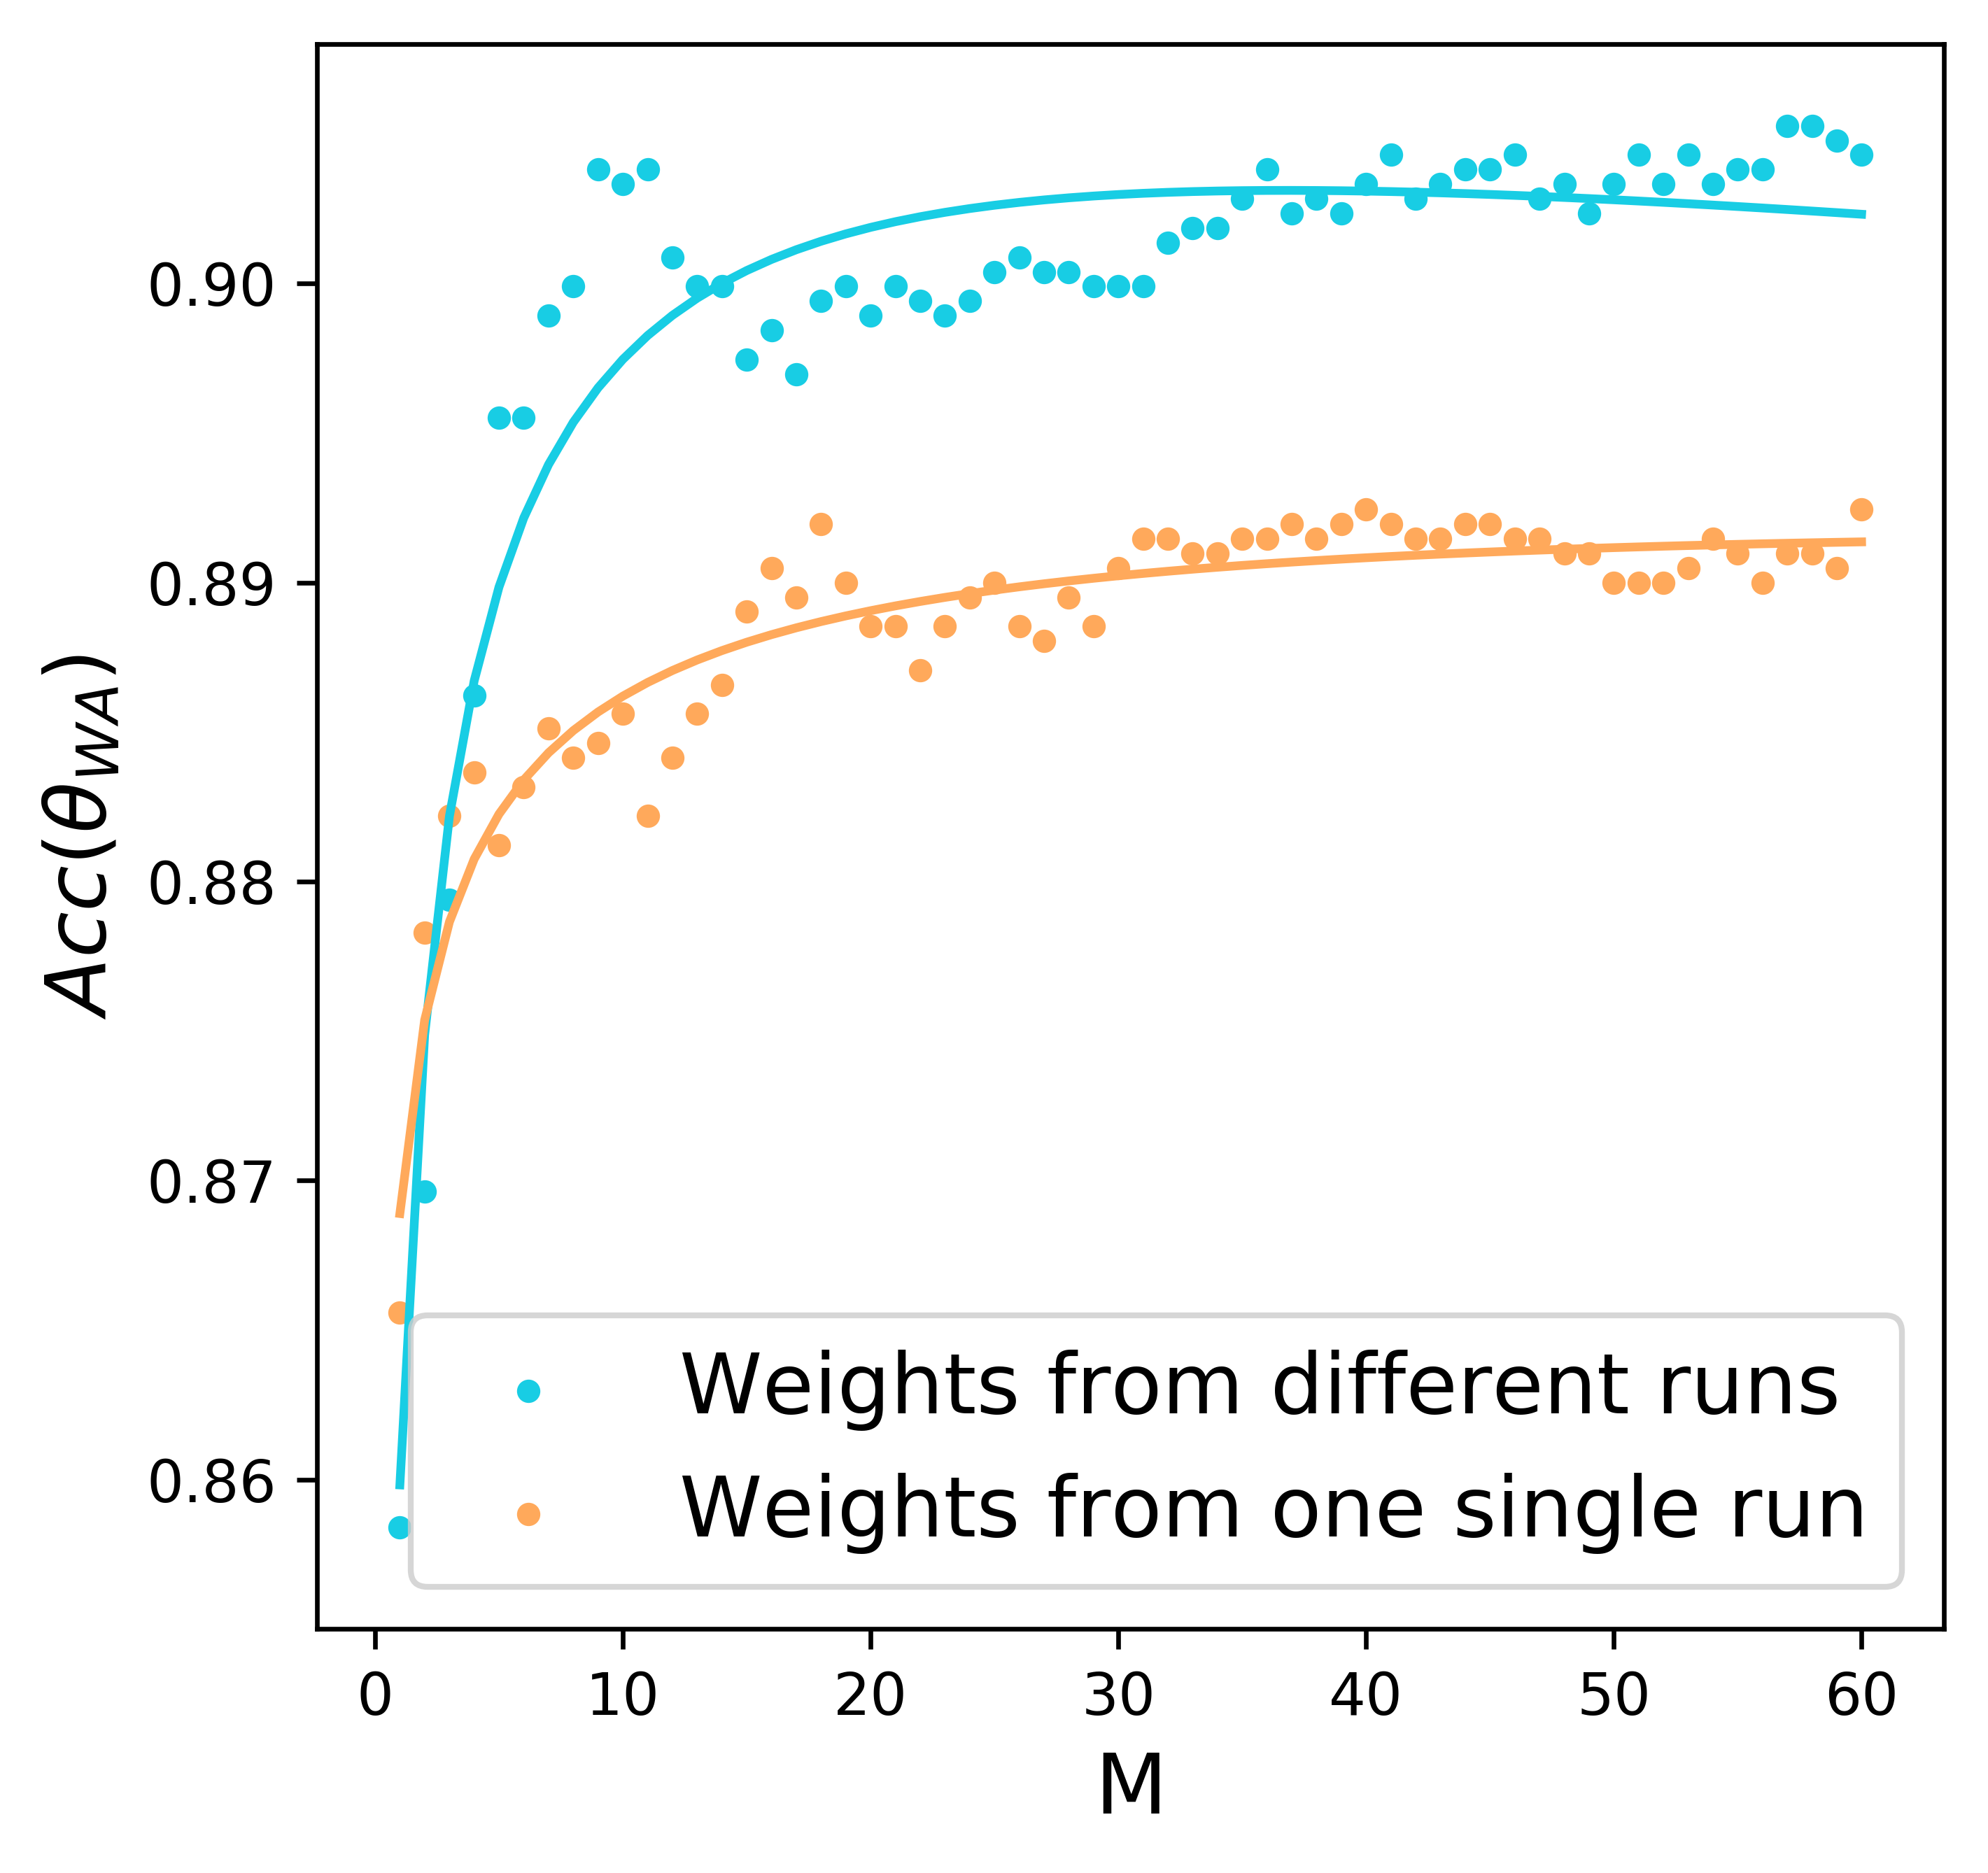
\includegraphics[width=0.9\textwidth]{pictures/files/final/pacs0_samediffruns_m_soup_ood.png}%
        \caption{Same as \Cref{fig:home0_m_vs_acc}.}
    \end{subfigure}
    \label{fig:same_analysis_pacs}%
    \caption{Same analysis on PACS as previously done on OfficeHome.}%
\end{figure}%


\section{\reb{Number of training runs}}

\label{app:valueofm}

\reb{In our experiments, we train $20$ independent training runs per data split. We selected this value as $20$ is the standard number of hyperparameter trials in DomainBed \cite{gulrajani2021in}. In \Cref{fig:home0_valueofm} we ablate this choice on the OOD domain \enquote{Art} of OfficeHome. We observe that a larger number of runs leads to improved performance and reduced standard deviation. These results are consistent with our theoretical analysis, as the variance is divided per $M$ in \Cref{prop:b_var_cov}. If reducing the training time is critical, one could benefit from significant gains over ERM even with a smaller number of runs: for example, $10$ runs seem sufficient in this case. This analysis complements \Cref{fig:home0_m_vs_acc} --- where $60$ runs were launched then sorted in increasing validation accuracy.}

\begin{figure}[H]
    \centering
    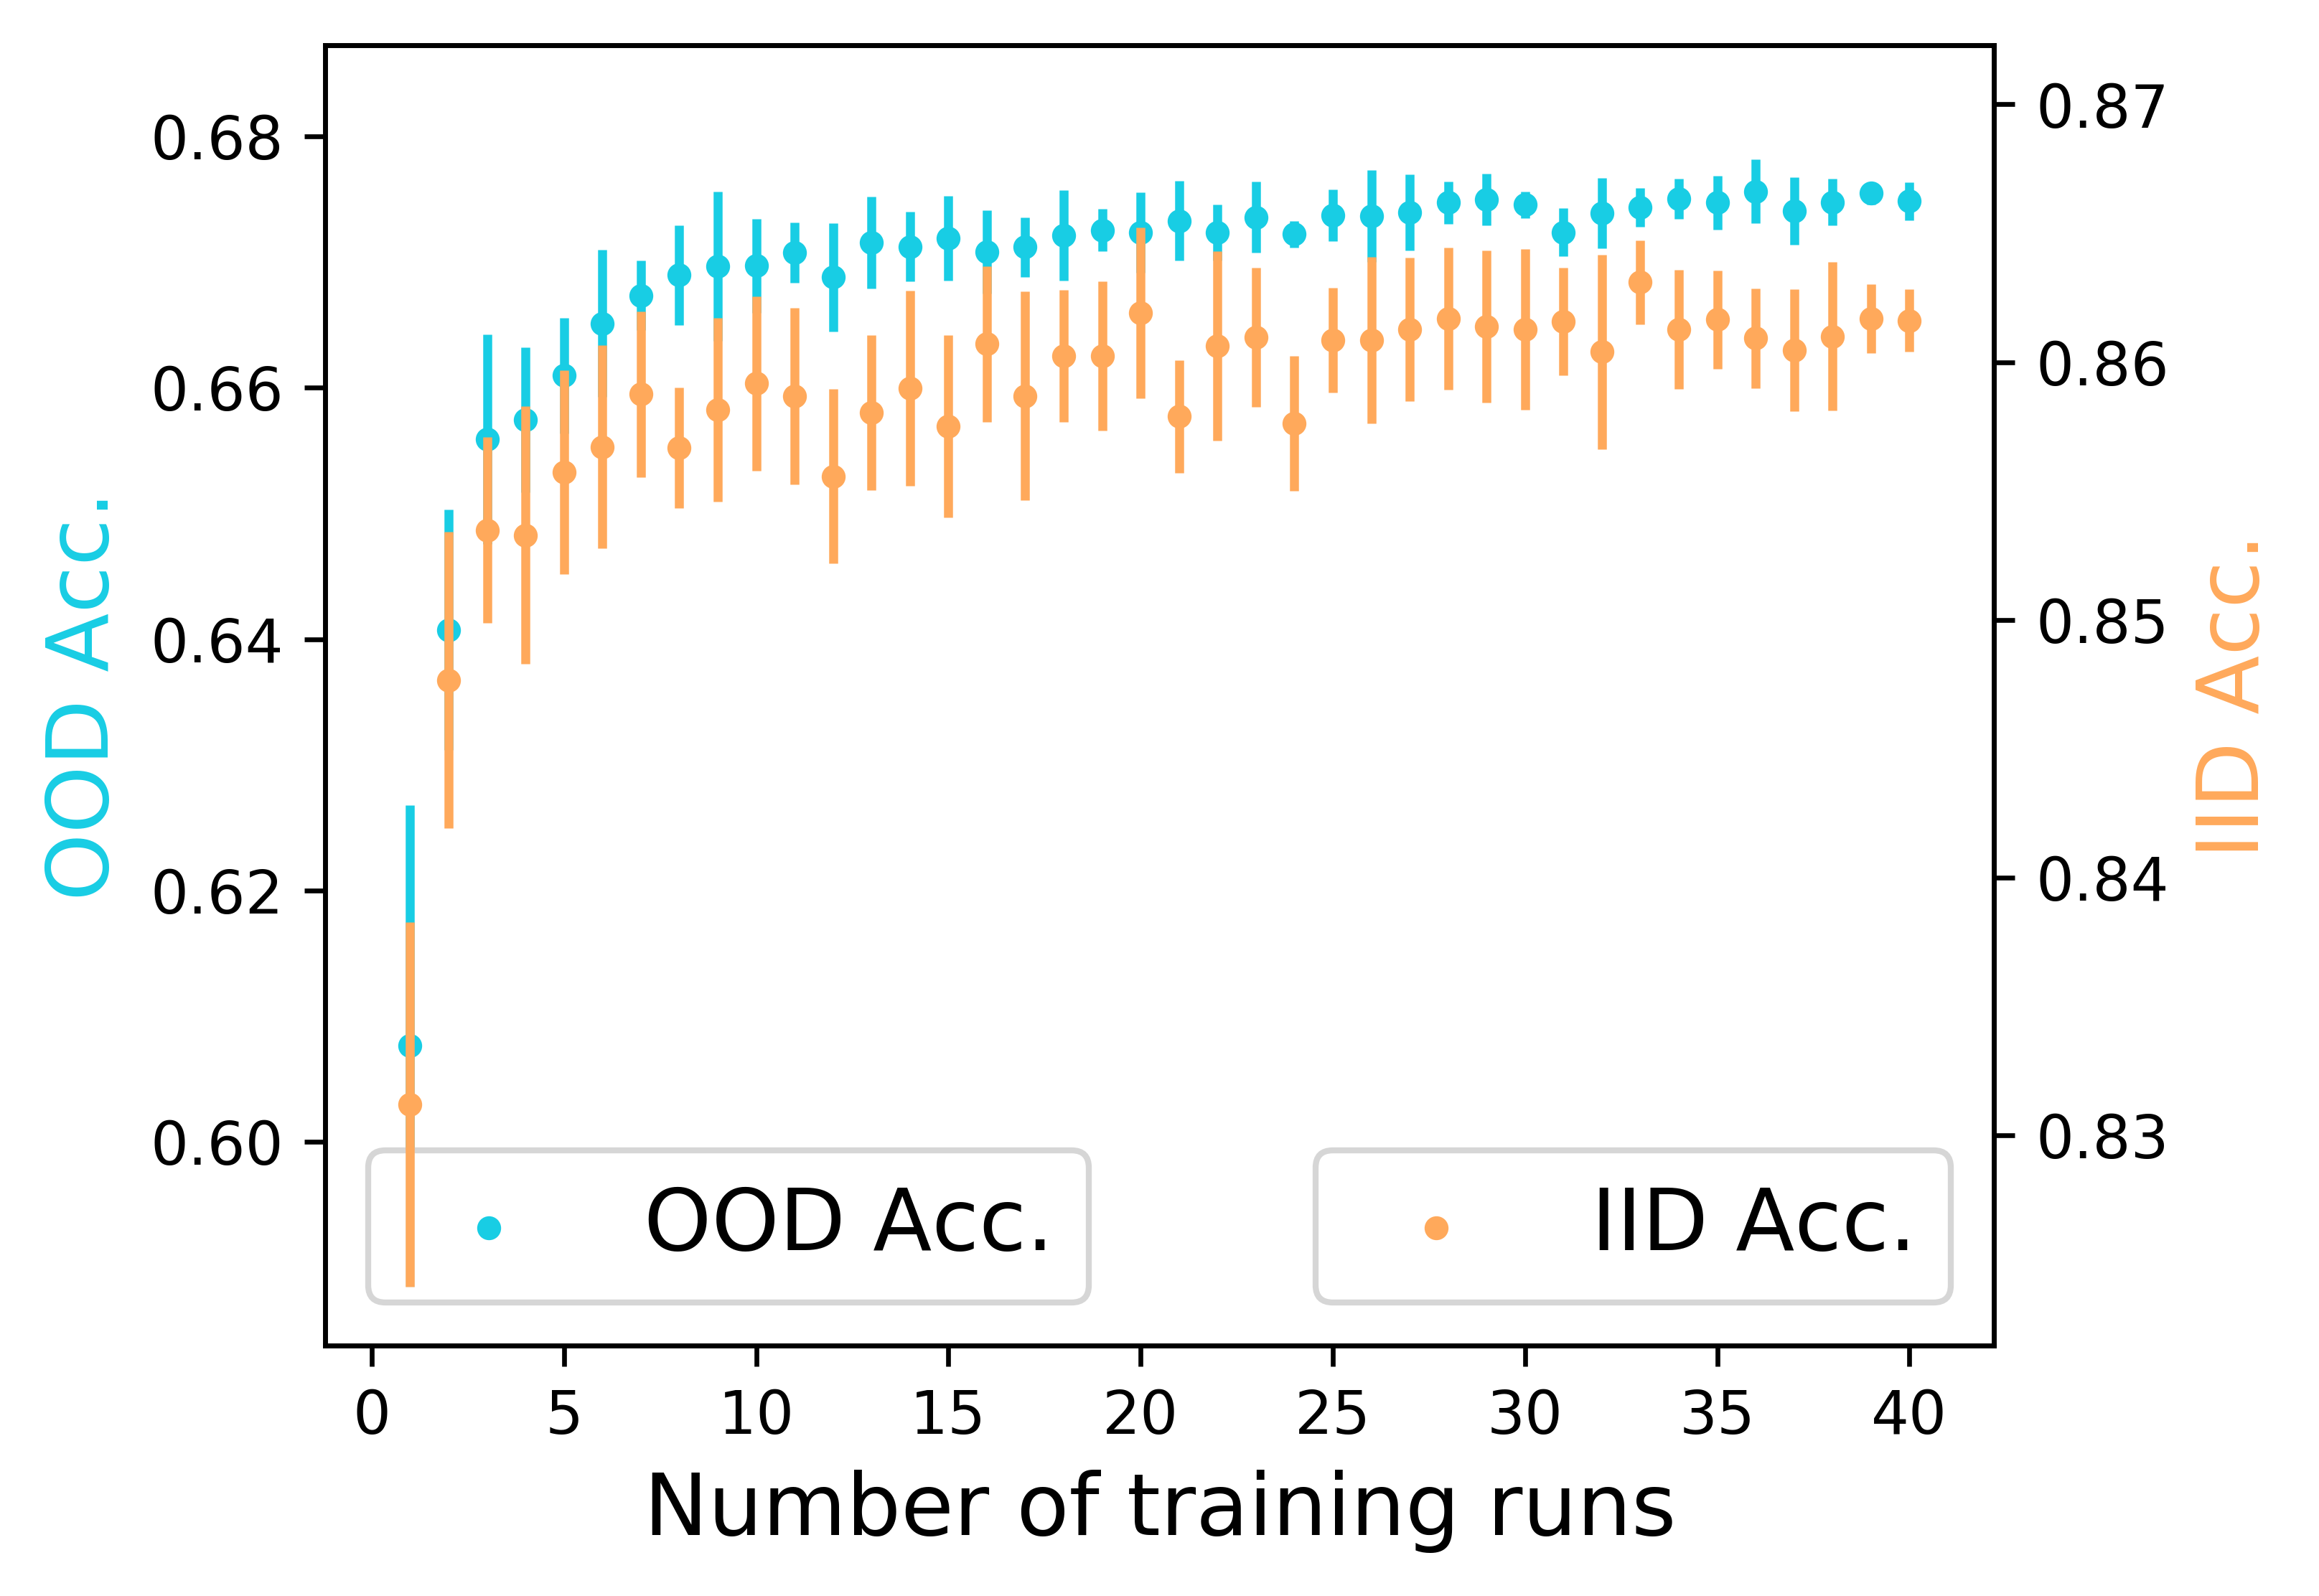
\includegraphics[width=0.5\textwidth]{pictures/files/final/diffruns_m_1to40_oodiid.png}%
    \caption{\reb{\textbf{Mean and standard deviation of DiWA-uniform's accuracy ($\uparrow$)} on OfficeHome when increasing the number of training runs and uniformly averaging all weights. \ood accuracy is computed on domain \enquote{Art}, while \iid accuracy is computed on validation data from the \enquote{Clipart}+\enquote{Product}+\enquote{Photo} domains.}}
    \label{fig:home0_valueofm}%
\end{figure}


\reb{Moreover, in \Cref{tab:m5} we report DiWA's results when considering only $5$ runs, with uniform weight selection. Interestingly, it shows that $M=5$ is enough to be competitive against SWAD \cite{cha2021wad}, the previous state of the art.}
\begin{table}[h]%
    \caption{\reb{\textbf{Accuracy ($\%, \uparrow$) on DomainBed}. DiWA-uniform and LP initialization \cite{kumar2022finetuning}.}}%
    \centering
    \adjustbox{width=1.0\textwidth}{
        \reb{\begin{tabular}{l|cccccc}
            \toprule
            \textbf{Algorithm}               & \textbf{PACS}  & \textbf{VLCS}  & \textbf{OfficeHome} & \textbf{TerraInc} & \textbf{DomainNet} & \textbf{Avg} \\
            \midrule
            SWAD \cite{cha2021wad}           & 88.1 $\pm$ 0.1 & \textbf{79.1} $\pm$ 0.1 & 70.6 $\pm$ 0.2      & 50.0 $\pm$ 0.3    & 46.5 $\pm$ 0.1     & 66.9         \\
            DiWA: $M=5$              & 87.9 $\pm$ 0.2 & 78.3 $\pm$ 0.3 & 71.5 $\pm$ 0.2      & 51.0 $\pm$ 0.7    & 46.9 $\pm$ 0.3     & 67.1         \\
            DiWA: $M=20$             & 88.7 $\pm$ 0.2 & 78.4 $\pm$ 0.2 & 72.1 $\pm$ 0.2      & 51.4 $\pm$ 0.6    & 47.4 $\pm$ 0.2     & 67.6         \\
            DiWA$^{\dagger}$: $M=60$ & \textbf{89.0}           & 78.6           & \textbf{72.8}                & \textbf{51.9}              & \textbf{47.7}               & \textbf{68.0}         \\
            \bottomrule%
        \end{tabular}%
    }}%
    \label{tab:m5}%
\end{table}%

